\documentclass[pageno]{jpaper}
%\usepackage{latex8}

% \usepackage[margin=1in]{geometry}
\usepackage{amsmath,amsthm,amssymb}
\usepackage{enumerate}
\usepackage{bbold}
\usepackage{graphicx}
\usepackage{multirow}
\usepackage{hhline}
\usepackage{color}
\usepackage{tsgcomments}

%******************************************************************************
% Anonymization Macros
% Usage : \ifanonymized{anonymized}{notanonymized}
% Uncomment one of the following

\newcommand{\ifanonymized}[2]{#1} % Anonymized
% \newcommand{\ifanonymized}[2]{#2} % Not Anonymized
%******************************************************************************

% Space optimization. cut lower priority first.
% use to mark parts that are nice to have, but cut due to space
\newcommand{\cut}[1]{} 

% use to mark parts that can potentially be cut
\newcommand{\optional}[1]{#1} 


\pagestyle{empty}

\setlength{\pdfpagewidth}{8.5in}
\setlength{\pdfpageheight}{11in}

\begin{document}

\title{
\vspace{-0.1in}
    Timing Compartments: An Architecture Primitive for Complete Software 
    Isolation
}

\ifanonymized{
    \author{}
}{
    \author{
    Andrew Ferraiuolo, Yao Wang, and G. Edward Suh\thanks{The first two authors 
    contributed equally to this work.}\\
    Cornell University\\
    Ithaca, NY 14850, USA\\
    \{yw438,af433,gs272\}@cornell.edu
    }
}


\date{}
\maketitle

\thispagestyle{empty}

\begin{abstract}

    %TODO

\end{abstract}

\section{Introduction}

Timing channel attacks are becoming a major threat as hardware is increasingly 
consolidated and shared by distrusting entities, which traditionally have been
isolated on their own physical machines. For example, in cloud computing, mutually distrusting 
parties own virtual machines on shared hardware. In mobile devices, users often
run downloaded applications that cannot be trusted often handle private personal
information.
While untrusted applications can be sandboxed using
traditional access control mechanisms to limit explicit communications,
timing 
channels can still be used by a malicious program to extract or leak secrets.
%from other co-located applications.
Further, unlike physical side-channel attacks such as power analysis that require
physical proximity, timing channels can be exploited in software by remote
adversaries.

%For example, end users download untrusted 
%applications from the Internet which can then execute on the same hardware as 
%software that will handle the user's sensitive financial data. System on chip 
%platforms tightly integrate hardware designed by directly competing companies.  
%This necessitates hardware sharing among the drivers and proprietary algorithms 
%owned by these distrusting companies. 
%So timing channels 
%vulnerabilities are not only prevalent, but easy to exploit.

%Many of the systems that are vulnerable to timing channels do take security 
%measures to prevent explicit channel attacks. In a cloud platform, the 
%hypervisor performs physical address translation on behalf of the virtual 
%machines to isolate the virtual machines in the physical memory. Hypervisors 
%also use access controls to isolate virtual machines, typically relying on 
%hardware abstractions such as protection rings. However, these security 
%mechanisms are not enough. They do nothing to prevent coresident VMs from 
%leaking secret information through timing channels induced by hardware sharing.

In this paper, we investigate an architecture abstraction, named timing compartments (TCs),
which allows software to explicitly request strong timing isolation among software
entities that share a multi-core processor.
The goal of timing compartments is to remove fine-grained microarchitecture-level timing interference
that cannot be controlled in software and enable strong timing isolation that is
comparable to running a software entity on its own processor.
The timing compartment is designed to prevent both unintentional information leaks
through side channels and intentional leaks through covert channels.
%Using the timing compartments, software designers can specify a timing protection
%requirement that is necessary for each application. 
%More importantly, 
When coupled with software-level protection mechanisms to control timing channels 
through coarse-grained events such as scheduling and I/O, timing compartments
can enable comprehensive timing isolation of program or a virtual machine.

The timing compartment is designed so that timing isolation can be
separated from traditional access control. For example, multiple programs or
virtual machines that are isolated from each other using virtual memory may
be grouped into a single timing compartment if they either belong to the 
same trust domain or do not require timing channel protection. 
This separation provides a system the flexibility to only pay overhead for
timing channel protection when it is truly necessary.

To realize the timing compartments, a multi-core processor needs to be
re-designed to control inter-core timing interference in shared hardware
resources that cannot be efficiently controlled in software.
In this paper, we identify all resources that can be shared concurrently among
multiple cores on a typical multi-core processor, namely shared caches,
on-chip interconnect, cache coherence mechanisms, and off-chip memory controllers,
and augment each shared resource with a mechanism
to eliminate timing interference.

This ``full-processor'' protection study revealed new sources timing
channels on a multi-core processor that have not been studied yet.
For example, we found that interfaces between hardware modules and 
a cache coherence mechanism can lead to timing channels, and demonstrate
a covert channel attack using the coherence traffic interference.
The integration effort also showed that protection mechanisms need to
be carefully coordinated in order to avoid unnecessary inefficiencies.
To the best of our knowledge, this paper represents the first study
that implements comprehensive timing channel protection for a full 
multi-core microprocessor and evaluates the overhead.

%Recent studies have investigated mechanisms to prevent
%timing channels in various microarchitecture components, including
%shared caches \cite{icache,newcache,deconstructing,cachegames}, processor pipelines 
%\cite{pipelines}, branch predictors~\cite{branchpred,predictingbranch}, on chip 
%networks~\cite{yaonocs}, and memory controllers~\cite{ushpca14}.
%However, we found that the full timing channel protection for a multi-core
%processor requires more than simply integrating previous protection 
%mechanisms. Our study identified new sources of timing channels at
%interfaces between hardware modules and also found that protection
%mechanisms need to be coordinated together to avoid unnecessary inefficiencies.

%Ascend~\cite{ascend} considers external timing 
%channel attacks, but does not prevent timing channels due to shared resources.  
%Execution leases~\cite{execution_leases} provide an architecture abstraction
%that prevents external timing channels by bounding the execution time of a code 
%segment, but Execution leases do not prevent the internal timing channels 
%caused by shared hardware. GLIFT \cite{citation_needed} can be used to identify 
%timing channels, but does not prevent them. Further, the area, power, and 
%performance overheads are prohibitively large.

%Unlike previous work, timing compartments eliminate all internal timing 
%channels in a conventional microarchitecture. When combined with standard 
%access controls, timing compartments achieve the security of running mutually 
%distrusting software on separate hardware with some of the performance benefits 
%of sharing hardware. To the best of our knowledge, this is the first 
%architecture technique to reach this goal. This work is also the first to 
%experimentally evaluate the cost of applying timing channel protection to every 
%vulnerable component. Further, we show that integrating these protection 
%mechanisms to form a complete system with minimal performance overheads is 
%nontrivial and requires careful coordination. In the process of designing an 
%integrated timing channel protection system we identified two novel 
%microarchitectural timing channels. In addition to these contributions we 
%extend the taxonomy of timing channels and show how this taxonomy can be used 
%to identify techniques that can eliminate timing channels in any additional 
%components (e.g. accelerators).

The simulation results suggest that the performance overhead of supporting
timing compartments is relatively low, especially when the number of timing
compartments that simultaneously run is small.
%for the SPEC benchmarks. 
Even though
the timing compartments require shared resources to be statically 
allocated, the overall impact on the performance is limited by the fact
that the protection only affects infrequent cache misses and that modern
processors include large caches. 

The following summarizes the main contributions of the paper.

\begin{itemize}
\item The paper introduces a new abstraction that enables software to
explicitly remove microarchitecture-level timing interference on a multi-core.
The timing compartment enables new
applications that require strong timing isolation of software modules.
\item The paper identifies new timing channels on a multi-core processor,
including the one through cache coherence, and presents
comprehensive protection mechanisms for a full multi-core processor.
\item The paper shows how protection mechanisms need to be coordinated to
reduce the overhead of timing compartments.
\item The paper evaluates the performance overhead of the full-processor
timing channel protection, and shows that the overhead can be reasonable.
\end{itemize}

The rest of the paper is organized as follows.
Section 2 introduces timing compartments and 
presents example applications that can be enabled by strong timing isolation.
Section 3 identifies the sources of timing channels in a multi-core processor, and
describes protection mechanisms to eliminate them. 
Section 4 presents how the hardware protection mechanisms based on time-division
multiplexing need to be coordinated to reduce overhead.
Section 5 evaluates the proposed architecture. Section 6 discusses related
work, and Section 7 concludes the paper.

\section{Timing Compartments}

This section introduces a new architecture abstraction, named timing compartment.
We first discuss the type of timing channels that the timing compartment is designed
to prevent. Then, we define the timing compartment, describe our threat model,
and discuss application scenarios that the timing compartments can enable.


\subsection{Taxonomy of Timing Channels}

%    \begin{figure}
%        \begin{center}
%            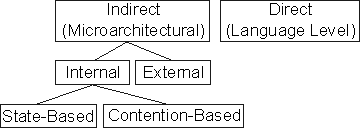
\includegraphics[width=2.2in]{figs/taxonomy.pdf}
%            \caption{The taxonomy of timing channels}
%            \label{fig:taxonomy}
%        \end{center}
%    \end{figure}

A timing channel represents a security vulnerability where the timing of events
depend on confidential information. An adversary can use timing channels as
side channels to learn secrets such as cryptographic keys or passwords or as
covert channels to intentionally bypass restrictions on communications.

%Figure~\ref{fig:taxonomy} summarizes the taxonomy of timing channels. \emph{Direct} or 
%language level timing channels can be identified by examining the source code 
%\cite{mitigation3}. A password checking algorithm that stops as soon as an 
%incorrect character is found causes a direct timing channel that leaks 
%information about the correct password. In contrast, \emph{indirect} or 
%microarchitectural timing channels cannot be identified in the source code 
%since they depend on hardware level behavior \cite{mitigation3}. Conventional 
%caches cause an indirect timing channel whenever the probability of a cache hit 
%depends on secret data. Programming language techniques have been developed to 
%address language level timing channels 
%\cite{timesens,mitigation1,mitigation2,mitigation3}. It is possible to reduce 
%the information leaked by some microarchitectural timing channels at the 
%language level \cite{mitigation3}. However, eliminating all leakage caused by 
%microarchitectural timing channels is difficult without hardware support.
%%%% More precise, wordier version:
%  However, efficiently providing strict timing-sensitive noninterference in 
%  the presence microarchitectural timing channels without the support of 
%  hardware is a hard problem.

Timing channels can be categorized into {\em external} and {\em internal} 
\cite{mitigation3}. 
External timing channels exist when the timing of a program's event that
can be observed externally leak information on data that the program processes. 
For example, a password checking program that sequentially compares strings
and stops on the first incorrect character leaks where a mismatch is.
As another example, Bernstein's attack~\cite{bernstein} exploits data-dependent
timing variations in a popular implementation of an AES encryption.
%Adversaries can carry out external timing channel attacks even without sharing 
%hardware with a victim program. 
Because the external timing channels happen when a program's operation differs
depending on a secret, language-level techniques have been developed to
mitigate them \cite{timesens,mitigation1,mitigation2,mitigation3}. 

%further divided into internal or 
%external timing channels. \emph{External} timing channels are not caused by 
%interference, and are exploited by an adversary that directly measures the 
%timing of the victim's actions. External timing channels can be exploited by an 
%adversary that does not share hardware with the victim. Bernstein's 
%attack~\cite{bernstein} exploits an external timing channel in popular 
%implementations of AES (such as OpenSSL). The external timing channel exists 
%because the cache access pattern both affects the overall execution time of the 
%AES implementation and depends on the secret key. The adversary carries out the 
%attack without sharing any hardware by directly measuring the response times of 
%the victim machine.
%%%%% The long explanation
% The adversary uses a copy of the same AES implementation as the victim to 
% time the encryption of a number inputs with a known key on the adversary's 
% local machine. Then, the adversary makes requests to the victim machine using 
% the same inputs and times how long the victim machine takes to encrypt the 
% inputs with an unknown key. In both cases, the execution time depends on the 
% cache access pattern which depends on the key. The adversary can use the 
% timing information gathered with the known and unknown keys to learn the 
% secret AES key.

Internal timing channels exist when one program's timing depends on another
program that shares the same hardware due to interference. In this case,
an adversary can exploit the timing channel by measuring the timing of its
own events even without directly observing a victim program.
For example, Percival~\cite{percival} showed an internal timing channel
through a shared cache where an attack program can extract an AES key
by measuring its own cache access time, which reflects a victim program's
cache accesses that depend on the key.



\subsection{Definition of Timing Compartments}

A timing compartment is a new architecture abstraction that allows software to
explicitly control {\em internal timing channels} that exist in shared systems. 
The ability to control timing channels, combined with a traditional access
control mechanism such as virtual memory, enables complete software isolation
because the timing channel is the only form of side/covert channels that can be
exploited in software without physical attacks.

From the software perspective, a timing compartment consists of one or more software 
entities such as threads, processes, and virtual machines. 
Then, software can express a policy that specifies which timing channels among
timing compartments are allowed or not. In general, the policy can take a form
of a lattice model, which defines ordering between security levels \cite{denning}.
This lattice model is quite expressive and widely used for information flow control. 
For example, the lattice may restrict timing channels only in one direction 
from $\mathtt{TC1}$ to $\mathtt{TC2}$ ($\mathtt{TC2} \leq \mathtt{TC1}$).
The lattice may disallow any timing channel between two compartments by making
them incomparable ($\mathtt{TC_1} \nleq \mathtt{TC_2}$, $\mathtt{TC_2} \nleq \mathtt{TC_1}$).

%Here, a software 
%entitiy is some system abstraction (such as processes or threads in a single OS 
%system or virtual machines in a virtualization based system) that execute 
%software and have an owner. Intuitively, a single timing compartment contains 
%only software entities that trust each other explicitly (such as all the VMs on 
%a machine owned by the same user) or implicitly (all the VMs that do not want 
%to pay for protection), and leakage within a timing compartment is safe.

Similar to other architecture abstractions such as virtual memory, the
timing compartments need to be implemented as a combination of hardware-software
mechanisms. The underlying hardware must provide mechanisms to distinguish
events from different timing compartments and control timing interference 
in shared resources.
Then, a trusted software component needs to manage the hardware mechanisms 
at run-time. We call this trusted software as timing compartment manager (TCM).

%To enforce the policy, a trusted software component called the timing 
%compartment manager (TCM) confines software entities into TCs. The TCM then 
%informs the hardware of the TCs and policy. At runtime, the TCM tags software 
%requests for hardware to indicate the TC of the software entity that made the 
%request. The hardware then enforces the policy by controlling how requests from 
%different TCs share resources.

The timing compartments allows software to explicitly control timing channels
among groups of software entities, but does not enforce any restrictions within
each compartment. We believe that handling timing channels separately from
traditional isolation abstractions such as processes and virtual machines is essential
to allow efficient system designs. Because timing channel protection is more expensive
than traditional access control, a designer should be able to pay the overhead
of timing control only when truly necessary.

%Timing compartments only address timing channels; they do not control 
%information flow through explicit channels. Handling these concerns separately 
%allows for more flexibility in the overall system design.  When designing a 
%secure system, implementors must consider how the cost required to carry out a 
%particular attack compares with other attacks, the potential damage that could 
%be caused by an attack, and the cost and performance impact of implementing the 
%security mechanisms needed to stop it. This enables timing compartments to 
%provide timing channel protection only to software entities that need it.

\subsection{Threat Model}

%Goal
The goal of the timing compartment is to enable complete software isolation
on shared hardware, comparable to having separate hardware for each.
%Assumptions
In that sense, we assume that a target system has multiple cores with shared
resources such as caches, on-chip interconnect, and off-chip memory that can
be used by multiple programs concurrently. The system can also be time multiplexed.
%The multicore system of interest consists of hardware resources that are
%concurrently shared by multiple software entities. It is possible for software 
%entities to be time multiplexed on the same core (e.g.  by context switching 
%VMs), but the system does not allow software entities to execute concurrently 
%on the same core (e.g. through simultaneous multithreading). 
We also assume that there exists a trusted software layer such as an OS or a hypervisor,
which provides conventional software isolation for explicit communication channels.
The timing compartment manager (TCM) is assumed to be a part of this trusted software.

%Attacks we handle.
%However, these approaches to isolate software do not address timing channels 
%that leverage shared hardware. To guarantee total isolation, internal timing 
%channels must also be eliminated. We eliminate all internal microarchitectural 
%timing channels including state and state-based timing channels. 
%This includes 
%all timing channels caused by concurrently shared resources as well as timing 
%channels in hardware that is shared through time multiplexing (e.g. by context 
%switching).

The timing compartment aims to eliminate {\em internal} timing channels through
interference in shared microarchitecture resources. In particular, the goal is
to prevent both unintentional (side channels) and intentional (covert channels)
information leaks.
However, external timing
channels, which exist even with dedicated hardware, are not prevented by the
timing compartments. If necessary, the external timing channels can be controlled 
in software. 
Similarly, timing channels through I/O devices are not considered in this study
because their accesses can be controlled in software.
Finally, we not consider physical attacks on the system such as
physical side-channel attacks through power consumption or electromagnetic emission. 

%Attacks we don't handle.
%Since our goal is to address vulnerabilities 
%caused by hardware sharing,
%timing channels that are external to the hardware are not addressed.
%Any timing channels that are external to the hardware in this system would also 
%be present if the software entities executed on separate hardware. If 
%necessary, external timing channels can be controlled in software. Similarly, 
%we do not address language level timing channels since these may also be 
%addressed in software.  Lastly, we do not consider physical attacks and assume 
%that the adversary does not have physical access.


\subsection{Application Scenarios}

The ability to control internal timing channels can significantly increase a level of
assurance in a number of applications where distrusting entities share a
physical system. Here, we briefly discuss representative applications.

\subsubsection{Bring Your Own Device (BYOD)}

As mobile devices such as smartphones and tablets are becoming widely used, 
companies and government organizations are starting to allow employees to
use their own devices to access corporate data. This trend is often called
Bring Your Own Device (BYOD). However, there is a major concern that such a
mixed use can lead to a leak of confidential data through personal emails or
downloaded applications. Today's BYOD solutions such as Samsung Knox uses
software containers or virtualization to separate the two environments:
personal and work. Yet, these solutions cannot prevent information leaks
through internal timing channels.

\begin{figure}
    \begin{center}
        \includegraphics[width=1.51in]{figs/app_byod.pdf}
        \caption{A BYOD example.}
        \label{fig:app_byod}
    \end{center}
\end{figure}

The timing compartment enables a strong isolation guarantee in the BYOD
scenario. For example, consider the solution based on virtualization as 
shown in Figure~\ref{app:byod}. In this case, the virtual machines for
work and personal use can be assigned to two different timing compartment:
$TC_{work}$ and $TC_{pers}$. Then, the lattice can be set so that no
information can flow from $TC_{work}$ to $TC_{pers}$.
Note that the BYOD application only requires two timing compartments even
though a system may have many cores and run many applications.

\subsubsection{High-Assurance Cloud Computing}

In cloud computing such as Amazon EC2, virtual machines (VMs) from multiple
distrusting clients often share physical machines. 
%A cloud provider 
%co-locates many VMs on a single machine to increase its utilization,
%and tenants often have little control over where their VMs run. 
For example, a tenant may share hardware with competitors or attackers that 
want to extract sensitive data. Today's virtualization technologies restrict 
explicit communication channels among virtual machines, but cannot control 
internal timing channels. In fact, recent studies have shown that timing channels
can be exploited in commercial clouds to extract secrets such as 
a password \cite{FIXME}.
For some clients, timing channels may not be a major concern. Yet, for enterprise
or government clients who require high assurance, this security threat makes
public cloud computing not an option. 

\begin{figure}
    \begin{center}
        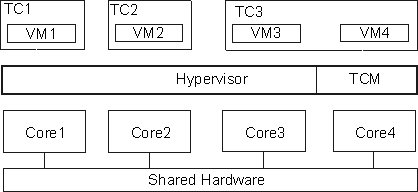
\includegraphics[width=2.79in]{figs/cloud_tcs.pdf}
        \caption{A cloud computing example. VM1 
        and VM2 have high security requirements, but VM3 and VM4 do not.}
        \label{fig:cloud_tcs}
    \end{center}
\end{figure}

The timing compartment can enable high assurance cloud computing by ensuring that
there cannot be unintended information leak among virtual machines.
Figure~\ref{fig:cloud_tcs} shows an example with four virtual machines (VMs).
%that have different security requirements. 
VM1 and VM2 require a strong isolation guarantee and distrust other VMs.
VM3 and VM4 run low-security applications that are not concerned with timing channels
but require high performance. The figure shows that three timing compartments can
be used to meet the security requirements in this example.
VM1 and VM2 are placed in their own timing compartments $TC1$ and $TC2$, but 
VM3 and VM4 are grouped in $TC3$. The lattice can be set so that VM1 and VM2
cannot leak information to any VM but no constraint is put on VM3 and VM4:
$TC3 \leq TC1, TC3 \leq TC2, TC1 \nleq T2, TC2 \nleq TC1$.
%TC3 preceeds both TC1 and TC2 implying timing channel leakage from VM3 or VM4 to 
%any other VM is not controlled. However, VM1 and VM2 cannot leak information to 
%VM3 or VM4. Additionally, VM1 and VM2 cannot leak information to each other 
%since TC1 and TC2 are incomparable. This meets the security requirements of VM1 
%and VM2 since both are totally isolated from the other VMs through timing 
%channels. Since VM3 and VM4 share a timing compartment, they can share 
%resources normally and incur minimal performance overheads.


\subsubsection{Untrusted Software} 

The ability to completely eliminate timing channels enables timing compartments
to be used to contain information even when software is potentially malicious.
For example, today's smartphone users often rely on many third party applications
that cannot be fully trusted to manage private or sensitive data. A system may
sandbox an untrusted application and restrict its communication channels
when it accesses sensitive data. However, today's access control mechanisms cannot
prevent the untrusted application from leaking information to another unrestricted
application through internal timing channels. The timing compartment can be added 
to provide a complete sandbox. 
In the cloud computing context, the same timing channel protection can be used
by a cloud provider to sandbox a third-party web services that cannot be fully trusted.

\subsubsection{Safety-Critical Systems}

In addition to protecting confidential data, the capability to control interference
in shared hardware can also be used to provide timing guarantees on safety-critical systems.
For example, hard real-time systems such as automotive controllers must meet
strict timing requirements. Unfortunately, today's multi-core processors provide
no timing guarantee when shared by multiple programs. The timing compartment can be
used to ensure that the timing of safety-critical components are not affected by
the rest of a system.


\section{Microarchitecture-Level Protection}

This section discusses internal timing channels in typical
multi-core processors and mechanisms to control them.

\subsection{Baseline Architecture}

    \begin{figure}
        \begin{center}
            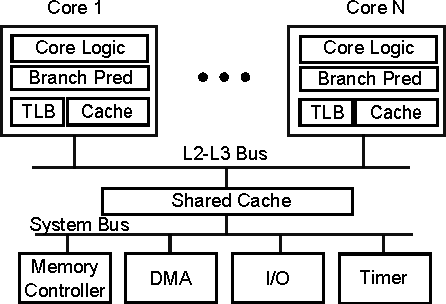
\includegraphics[width=3.04in]{figs/baseline.pdf}
            \caption{Baseline multi-core architecture.}
            \label{fig:baseline}
        \end{center}
    \end{figure}

Figure \ref{fig:baseline} shows a baseline multi-core architecture that we
extend with timing compartments in this paper. The architecture
has multiple cores, each with a core pipeline, a branch predictor, a TLB,
and one or more private caches. 
The cores are connected to a shared cache via an on chip network. A shared system 
bus connects the shared cache to a memory controller that manages requests to 
main memory.
We assume that each core may be time shared by multiple timing
compartments, but only one timing compartment, which we say is active, may run on each core
at a time. This assumption can be relaxed if timing channel protection
is added to per-core resources.

\Ed{Perhaps move all the assumption that we make here?}

%A trusted software layer (such as 
%an operating system) allocates software entities (such as processes) to the 
%cores. 

\subsection{General Protection Approaches}
\label{sec:general_approaches}

Here, we present a classification of internal microarchitectural timing channels 
and a framework of general solutions to address each type.
We follow these approaches to design our
protection mechanisms. These approaches also provide guidelines to
develop new protection mechanisms for components that are not included in
our baseline architecture.

\subsubsection{TCID}

The hardware protection mechanisms track which timing compartment originated 
each request and handle the requests accordingly. Each core has a register that 
stores the timing compartment ID (TCID) of the TC currently active on that core. This is used to derive 
the tags that are appended to requests originating from that core. The TCID is 
$log\ n$ bits where $n$ is the number of cores in the processor.
Events such as network packets or cache accesses that use shared resources are 
tagged with the TCID of the corresponding core. 
The timing channel protection mechanisms use this TCID to distinguish accesses
from among different timing compartments.

\subsubsection{Classification of Internal Timing Channels}

There exists an internal timing channel from one entity (say $E1$)
to another ($E2$) whenever the timing of an action of $E1$ can be affected 
by the behavior of $E2$.

There are two types of such timing channels in hardware: state-based
and contention-based.
A \emph{state-based} timing channel occurs whenever there is a state element 
with an access time that depends on its content and that state element is 
shared among multiple entities.
For example, a conventional shared cache has state-based timing channels, because 
its cache hits are faster than misses.
A \emph{contention based} timing channel occurs whenever multiple entities 
share a resource that can handle only finitely many requests at a time.
Conventional buses have contention-based timing channels.

\subsubsection{State-Based Timing Channel Protection}

%Caches, TLBs, and branch predictors all have state-based timing channels. 
%In 
%each, requests that use an entry that is present in the state elements (e.g.  
%cache hits) are faster than requests to entries not present (e.g. cache 
%misses). The state elements can contain a finite number of entries, so entries 
%must be evicted and replaced with new ones. One software entity can evict 
%entries owned by another, causing interference and timing channel leakage if 
%the choice of entries evicted correlates with a secret. 
In general, the state-based 
timing channels can be removed by applying flattening, partitioning, or 
flushing.
Flattening eliminates the dependence of access time on the state by forcing 
every access to finish in the same (worst case) time. For example, to remove timing 
interference in the row buffers of DRAM, all DRAM accesses may be treated as 
a row buffer miss.
For some components, this is a 
brute-force approach. Applied to caches, every access must be treated as a 
miss, so this is equivalent to removing the cache. 

Partitioning removes interference by ensuring that each entity can
only affect a disjoint subset of state elements. The partitions
should not change dynamically depending on the run-time demands of entities.
In the simplest case, partitions can be static.
However, partitions do not need to be homogeneous and can be sized according 
to static performance characterizations of each software entity (assuming this 
information can be made public and does not depend on secrets).

%prevents software entities that share state elements from 
%interfering. Static partitioning is realized by dividing the state elements 
%into separate partitions for each software entity. Entities are only allowed to 
%evict entries within their own partitions. Partitions must either be static, or 
%at least not resized or moved based on the dynamic behaviour of an entity.
%% If a partition is increased for an entity intensively using the state 
%% elements, the other entities can detect that their partitions have been 
%% resized and information is leaked.
%However, partitions do not need to be heterogeneous and can be sized according 
%to static performance characterizations of each software entity (assuming this 
%information can be made public).

Flushing can remove state-based timing channels for a resource that is time-shared.
For example, a branch prediction table may be cleared on a context switch.
%At the end of a time quantum, the state elements are completely cleared before 
%passing ownership of the state elements to the entity in the next time quantum.  
%Resources that can be flushed can also be partitioned, and there are tradeoffs 
%between these approaches.
% Flushing increases the time wasted at the end of a time quantum if flushing 
% cannot be done in less than one clock cycle. Clearing the state between time 
% quanta also increases the number of slower accesses at the start of the 
% quanta (e.g. it causes more cold cache misses). However, partitioning reduces 
% the total number of state elements that can be allocated to each entity. 
In general, there is a trade-off between partitioning and flushing.
For long time slices (e.g. when context switching is infrequent), 
flushing is preferable because it allows the full capacity to be used by
each timing compartment. In contrast, partitioning may
offer better performance for short time slices by reducing cold misses.
%time to reload
%the state on a context switch.

\subsubsection{Contention-Based Timing Channel Protection}

%Contention based timing channels arise whenever a resource that is shared among 
%multiple software entities can only handle a finite number of requests at a 
%time. 
Contention based timing channels can be removed by duplication or by
time division multiplexing (TDM). Duplication removes interference by
allocating dedicated resources for each timing compartment.
However, this has obvious area overhead implications. If 
duplication is infeasible, time division multiplexing can be used.
%TDM 
%defines a schedule where each software entitiy is guaranteed a period of time, 
%called a time quantum, where only that entity can use the resource. The 
The schedule of time slices must either be static or independent of the 
dynamic behavior of software entities.

%\subsubsection{External Timing Channel Protection}
%
%Though external timing channels are outside the scope of this 
%paper, there are a class of timing channels that are internal to hardware, but 
%appear as external timing channels between two software entities. This form of 
%external timing channel exists in systems where distrusting software entities 
%must communicate. For example, one software entity might be a user space 
%process and another might be a process that performs only high-assurance 
%operations. The user space process requests the high-assurance process to 
%perform some operation on its behalf. The user space process can directly 
%observe the execution time of the other process. This type of timing channel 
%can be solved in software by forcing the observable execution time to 
%equal the worst case execution time, stalling if necessary.


\subsection{Full-Processor Protection}

Timing compartments use hardware mechanisms that control all internal timing 
channels in a microprocessor. Designing a full processor with timing channel
protection may seem rather straightforward. In our baseline architecture, there are
only three main structures that are shared concurrently: a shared cache, on-chip
buses, and a memory controller. Moreover, recent studies have proposed mechanisms
to control timing channels in each of them. For example, researchers have proposed
statically partitioning the shared cache \cite{percival}, and using time division 
multiplexing with a fixed schedule for the on-chip interconnect 
\cite{yaonocs, surfnoc} and the memory controller \cite{ushpca14}.

%Many microarchitectural timing channels and corresponding solutions are 
%well-known. Shared caches create a state-based timing channel where interfering 
%entities cause cache block replacements. This can be prevented by partitioning 
%the cache among the entities. On chip networks and buses have
%timing channels since only one entity can use the bus at a time. Time division 
%multiplexing can resolve this issue \cite{yaonocs}. The authors of 
%\cite{ushpca14} have exposed timing channels in the main memory and memory 
%controller. They propose time division multiplexing the memory controller, 
%partitioning the memory controller queueing structure, and using a closed-page 
%row buffer management policy to close these timing channels. 
%%%%% It isn't totally obvious that private resources are actually shared, and 
%%%%% we don't have a citation for this, so maybe it doesn't need to be here..
% Finally, the private, per-core resources of the system such as the branch 
% predictors, TLBs and private caches also create timing channels since 
% software entities share cores through time multiplexing (for example, 
% processes may be context switched in and out of the same core). These can be 
% resolved by flushing the state elements of these resources on before moving a 
% new software entity onto the core.

However, achieving secure and efficient timing channel protection on a full processor
requires much more than simply putting known protection mechanisms
together. During the design process, we found three new sources of timing channels
in module interfaces that were not discussed previously, and found a bug in the
memory controller protection \cite{ushpca14}.
%The cache protection scheme also needed to be slightly changed to handle cases when timing
%compartments have shared memory pages. 
We also found that time multiplexed
microarchitecture structures must be carefully coordinated in order to avoid 
unnecessarily high overheads. 
%%%%% We have not demonstrated total starvation in practice or on paper.
% or total starvation.

The rest of this section provides a detailed list of timing channels in our
baseline architecture, and presents a protection mechanism that we use for each of them.
Table \ref{table:timing_chan_summary} summarizes these timing channels and
solutions. 
Then, the next section discusses how these protection mechanisms
need to be managed and coordinated together.
We note that the processor design here uses simple static protection
mechanisms that prevent timing channels in both directions. The mechanisms 
can be further optimized for efficiency.

\def\novelcolor{Green}
\begin{table*}
\begin{tabular}{l|l|l|l}
    \hline
    Component & Timing Channel & Classification & Solution\\
    \hline
    \multirow{3}{*}{Shared Caches}
    & Replacement & State  & Set Partitioning \\
    \hhline{~---}
    & {\color{\novelcolor}MSHRs}
    & {\color{\novelcolor}Contention }
    & {\color{\novelcolor}Duplicate MSHR Banks} \\
    \hhline{~---}
    & {\color{\novelcolor}Response Ports}
    & {\color{\novelcolor}Contention }
    & {\color{\novelcolor}Separate Queues \& Time Multiplexing}\\
    \hline
    \multirow{5}{*}{DRAM \& Memory Controller}
    & Page Faults & State  & Address Space Partitioning \\
    \hhline{~---}
    & DRAM Resources & Contention  & Time Multiplexing \\
    \hhline{~---}
    & Queueing Structure & State  & Partitioned Queue \\
    \hhline{~---}
    & Row Buffer & State & Closed Page Policy (Flattening)\\
    \hhline{~---}
    & {\color{\novelcolor} Response Ports} 
    & {\color{\novelcolor} Contention }
    & {\color{\novelcolor} Separate Queues \& Time Multiplexing}\\
    \hline
    \multirow{2}{*}{Network} 
    & Interconnect Contention & Contention & Time Multiplexing \\
    \hhline{~---}
    & Queueing Structure & State & Partitioned Queue \\
\end{tabular}
    \caption{Summary of timing channels and protection approaches. Green represents new timing channels that were not identified in previous work.}
    \label{table:timing_chan_summary}
\end{table*}

\subsection{Shared Caches}
\mbox{}\newline
\textbf{Cache State \& Replacement}
The shared cache causes state-based timing channel vulnerabilities, because accesses
from one timing compartment may evict the cache blocks of another timing compartment.
This state-based timing channel is the focus of prior cache timing channel 
studies.
%to the memory hierarchy for addresses that are stored in the cache (cache hits) 
%are returned faster than requests for entries not stored in the cache (cache 
%misses). So, the time required to access the cache depends on its state. The 
%cache can only accommodate a finite number of entries, so when new entries must 
%be stored, old ones are evicted. One software entity can evict the entries of 
%another, causing timing channel leakage.

Our design uses static cache partitioning to eliminate the cache
interference among timing compartments.
The cache state of different timing compartments are forced to reside in 
disjoint regions of the cache so that one timing compartment cannot evict the 
entries of another.
In general, there exist two approaches for cache partitioning:
way partitioning \cite{dynamic_partitioning} and
set partitioning \cite{rtas_cache_framework}. Way partitioning restricts
each compartment to only replace certain cache ways. Set partitioning
either uses page coloring or modifies the index function so that each compartment
only uses a subset of the cache sets. Both partitioning methods are equally
effective at removing timing channels. In our implementation, we used
set partitioning so that each compartment can benefit from full 
cache associativity.

%We note that the cache partitioning needs a special care if multiple timing
%channels shared the same physical memory location. In this case, a cache
%access from one compartment may hit in another compartment partition. Such a
%hit must be handled as a miss from the timing perspective. 


%Set associative caches divide 
%the cache into ways. Each way as a single slot for each cache set. A cache 
%block may be stored in any way, but the set it belongs to is determined by a 
%segment of its address bits called the index. Since many addresses are mapped 
%to the same set, another segment of the address, the tag, is used to detect 
%cache hits (i.e. if a specific address is present in the cache).

%Way partitioning allocates a subset of the ways to each entity 
%\cite{citation_needed}. This results in a reduction in the effective 
%associativity utilized by each entity, and thus, causes more conflict misses 
%and weakens performance. Set partitioning manipulates virtual to physical 
%address translation to restrict the sets that a particular entity can occupy.  
%When done at the granularity of a page, this is called page coloring, and this 
%has been proposed for performance \cite{citation_needed} and real-time systems 
%\cite{rtas_cache_framework}.  Although both techniques increase the number of 
%capacity misses, set partitioning does not increase the number of conflict 
%misses, so we chose this technique for our implementation.

\textbf{MSHR Contention}

We identified new internal timing channel vulnerabilities in the shared cache 
interface. The first, is caused by contention for the miss status holding 
registers (MSHRs) in non-blocking caches.
A non-blocking cache uses MSHRs to track information about in-flight cache misses 
(memory requests).
% With only a single MSHR, the system can tolerate a single outstanding cache 
% miss (hit under miss). With more MSHRs, it can tolerate multiple outstanding 
% misses (miss under miss). In any case, the system can tolerate only finite 
% outstanding misses at a time. 

The number of outstanding cache misses that the cache can tolerate depends on 
the number of MSHRs. Once all MSHRs are exhausted, the cache will stall on
a miss resulting in increased latency for cache accesses.
Therefore, shared MSHRs cause an internal timing channel, because one timing
compartment can delay accesses from another compartment by exhausting the MSHRs.
To remove the MSHR contention timing channel, our processor design duplicates
the MSHRs and dedicates MSHRs to each timing compartment.

\textbf{Response Port Contention}
The cache ports cause another contention-based timing channel yet to be 
discussed in the literature. Conventional caches have CPU-side ports and 
memory-side ports both of which are split into request and response ports. 
%On the cache miss path, the cache receives a request through the CPU-side request 
%port, and detects a miss. The cache issues a request to the memory through its 
%memory-side request port and then receives a response through its memory-side 
%response port. Finally, the cache responds to the CPU through its CPU-side 
%response port.
However, each port can only service a single response/request at a time
causing contention for these ports. For example, in a non-blocking cache,
data from an outstanding miss may be ready while a response for a cache hit
is being transferred through the CPU-side port.
It is also possible that the CPU-side bus is busy and will block the response
port. 
%Requests to the cache are controlled through the on 
%chip network, so any contention for this port may be controlled there. However, 
%there is uncontrolled contention in the CPU-side response port. Typically cache 
%accesses return more data than can be sent over a bus in a single cycle, 
%necessitating multi-cycle transfer (for example a cache block may consist of 
%several words and the bus may allow only a single word to be transferred each 
%bus cycle). Since the cache is nonblocking, it is possible for a response from 
%memory to return to the cache and require the cache response port while the 
%data from a cache hit is being transferred. 
To deal with this port contention, conventional caches include a shared queue
where responses can be buffered. Unfortunately, 
timing interference in either the cache ports or the cache response queue can
lead to an internal timing channel. To remove this timing channel, we apply
time division multiplexing to the cache ports and replace a shared queue with
smaller per-compartment queues.

\subsection{On-Chip Interconnect}

As pointed out by previous studies \cite{yaonocs, surfnoc}, shared on-chip 
interconnects
have contention-based timing channels because each link can be used by only 
one compartment at a time. In our processor design, we apply time
division multiplexing with a fixed schedule to both the bus between private
and shared caches and the bus between the shared cache and the memory controller.
For each time slice, accesses from only one timing compartment are allowed to
use the bus.

\subsection{Main Memory Controller}

The main memory is shared concurrently among multiple cores. As a result,
interference among memory accesses from multiple timing compartments can lead
to internal timing channels. 
%and 
%analogous to the timing disparity between cache hits and misses, page faults in 
%main memory take substantially longer than accessing entries that are present 
%in main memory. This timing channel can be handled simply by partitioning the 
%address physical address space for each entity.
%However, the memory controller has additional timing channels due to resource 
%contention as well as other state based timing channels. 
Wang et al. proposed a timing channel protection scheme for the shared memory
controller, which is based on time division multiplexing \cite{ushpca14}. 
We adopt their protection scheme in our processor design and briefly summarize 
the sources of timing interference and countermeasures here.
However, we found a minor vulnerability in their protection scheme and
adjusted the scheme to remove it.

\textbf{Request Queue}
A conventional memory controller has a queue for buffering memory requests until
they can be issued. This queue is typically shared among requests and creates
a contention-based timing channel, because requests from one compartment can block
requests from another. We remove this interference by placing the shared 
queue with smaller per-compartment queues, effectively duplicating the single queue.

\textbf{Row Buffer State}
There exists another state-based timing channel in the shared memory controller
if an open page policy is used. On a DRAM access, an entire row is read from
a memory array and stored in a row buffer (sense amplifier). If this buffer is
used as a cache, it creates a timing channel, because consecutive accesses to 
the same row are faster than accesses to different rows.
The protection scheme removes this timing channel by applying the closed page
policy, which precharges the row buffer after each access. This
closed page policy can be seen as an application of the flattening approach that
treats each access as a row buffer miss.
A previous study \cite{ushpca14} showed that the close page policy does
not have a noticeable performance disadvantage over the open page policy, because it
makes an access to a different row faster by performing a precharge early.

\textbf{DRAM Contention}
The DRAM device contains several resources such as the command bus, data
bus, banks, and ranks that can only service a finite number of requests at a time. 
Therefore, these cause contention-based timing channels.
%For example, two requests to the same bank cannot
%be scheduled at the same time. In a conventional memory controller, one request 
%would be delayed, causing interference.
% Suppose the queueing structure contains a request from a victim owned 
% software module for a bank. If an adversarial software module issues a 
% request to the same bank, it will be delayed, informing the adversary that 
% such a victim request exists. Similarly, contention for the command bus 
% causes a timing channel that may be observed in the scheduler. If a request 
% from one software module arrives at the scheduler in the same cycle as a 
% request from another software module and for a different bank, one of the 
% requests is scheduled and the other is delayed since only a single command 
% can occupy the command bus at a time.
The protection scheme uses timing division multiplexing (TDM) to remove these
timing channels. The TDM protection for main memory requires a special period 
in each time slice where no new
request can be issued in order to prevent in-flight requests or refreshes to
create timing interference.

%A surprising contention timing channel due to refreshes complicates TDM for 
%memory controllers. DRAM banks that are handling a request cannot be refreshed, 
%so refreshes are actually stalled by regular requests. This stall can shift the 
%refresh to the following turn and indicate that an access to that bank is 
%taking place. Since the refresh timing is public information, the dead time of 
%each time quantum where a refresh takes place is increased to guarantee the 
%refresh completes.

\textbf{Adjustments to the Protection Scheme}
During the process of integrating timing protection mechanisms for a full
processor, we found two vulnerabilities in the previously proposed scheme.
First, similar to the shared cache, the response port of a memory controller
can lead to a contention-based timing channel. We removed this channel by
separating queues for each timing compartment and applying TDM to the port.
Second, we found that the dead time proposed by ~\cite{ushpca14} was 
not sufficiently long. Previous work erroneously assumed that requests to two
different ranks would not interfere.

\subsection{Cache Coherence}
In a multi-core system, threads are running concurrently on different cores. These threads may share some
data which they read from or write to. The shared data thus can have multiple copies exist in each core's
private cache. In general, a cache coherence protocol is used to ensure each thread gets the most updated
data to work with.

In a snooping-based protocol, the caches on the same level are connected with a snooping bus. When a request
comes into a cache and incurs a cache miss, a snooping request is sent on the snooping bus. All the other
caches observe the snooping request, and one of them may respond to the request by forwarding the data if 
the data exists. The operations to handle snooping requests and responses highly depend on the specific cache 
coherence protocols being used. Commonly used protocols include MSI, MESI and MOESI~\cite{mark_book}.

% If different timing compartments share data, there is clearly a timing channel introduced by the cache coherence
% protocols. For example, TC0 wants to write to A, and A exists in TC1's cache. In order to perform the write, the
% cache coherence protocol will invalidate A in TC1's cache. Later when TC1 wants to read A, it will incur a cache
% miss which indicates TC0 has written to A. 
In our threat model, timing compartments are allowed to share some OS protected read-only data. This assumption
introduces a timing channel through the cache coherence protocols. Take MOESI protocol as an example, assume TC0 wants
to read a shared data A and incurs a cache miss, while A is in TC1's cache with an Owned(O) state. The MOESI protocol
will forward A to TC0's cache through the snooping bus, which shortens TC0's miss latency compared to accessing the
next level of cache. TC0 then knows A exists in TC1's cache and may correlate this fact with secret information. 
Even if there is no shared data between timing compartments, there still exists a timing channel through the cache
coherence protocol, because the snooping bus is shared by different timing compartments. 
The coherent traffic from different timing compartments can interfere on the snooping bus, thus introduce timing
channels, as demonstrated in the example below.

In this example, we conduct a covert channel attack through cache coherence protocol on a four-core system. 
The system configuration 
is shown in Figure~\ref{fig:coherent_system}. Each core has a private L1 and L2 cache, and the four cores share
the L3 cache. The four L2 caches are connected with a snooping bus which uses a MOESI protocol. 
In this example, there are two attackers who
want to communicate a secret data when the direct communication between them is strictly disallowed. Each attacker 
belongs to a different timing compartment. Attacker0 occupies core 0 and core 1 while attacker1 occupies core 2 and
core 3. 

\begin{figure}
    \begin{center}
        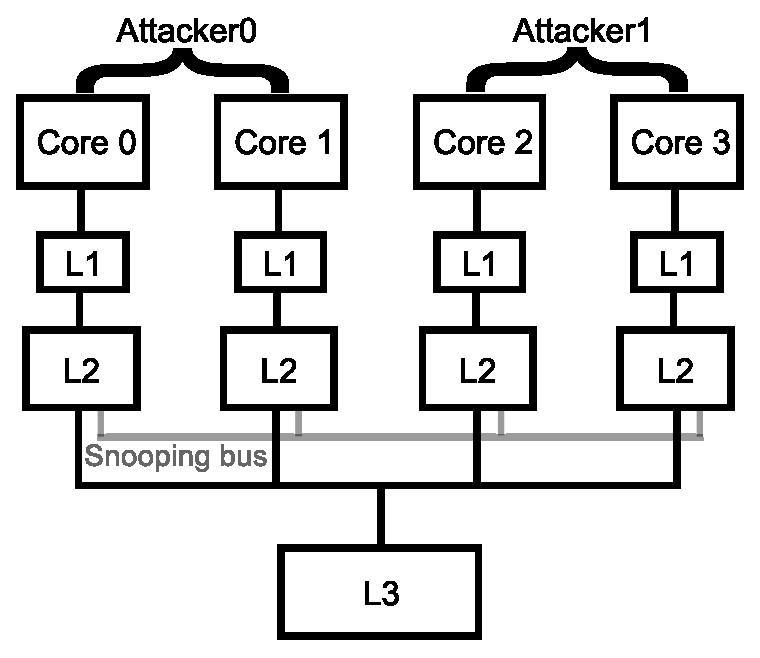
\includegraphics[width=2.3in]{figs/coherent_system.eps}
        \caption{System Configuration}
        \label{fig:coherent_system}
    \end{center}
\end{figure}

Attacker0 has two threads, each running on a different core. Both threads run a $for$ loop of 4000 iterations, and
write to a shared data in each iteration. Before each write is performed, one L2 cache has to forward the data
to the other L2 cache through the snooping bus and invalidates its own copy, according to the cache coherence protocol. 
As a result, there is a lot of coherent traffic between these two threads. Attacker0 runs this $for$ loop repeatedly and
records the time to finish the $for$ loop using c++ timing functions.

Attacker1 owns the secret data ('01101100') and tries to communicate this secret to Attacker0. It checks each bit
in the secret data. If the bit is 0, it executes a $for$ loop which writes to a data in each iteration. This does not produce 
coherent traffic. If the bit is 1, Attacker1 spawns a new thread, which also runs a $for$ loop that writes to the same data, hence producing a lot of coherent traffic. 

\begin{figure}
    \begin{center}
        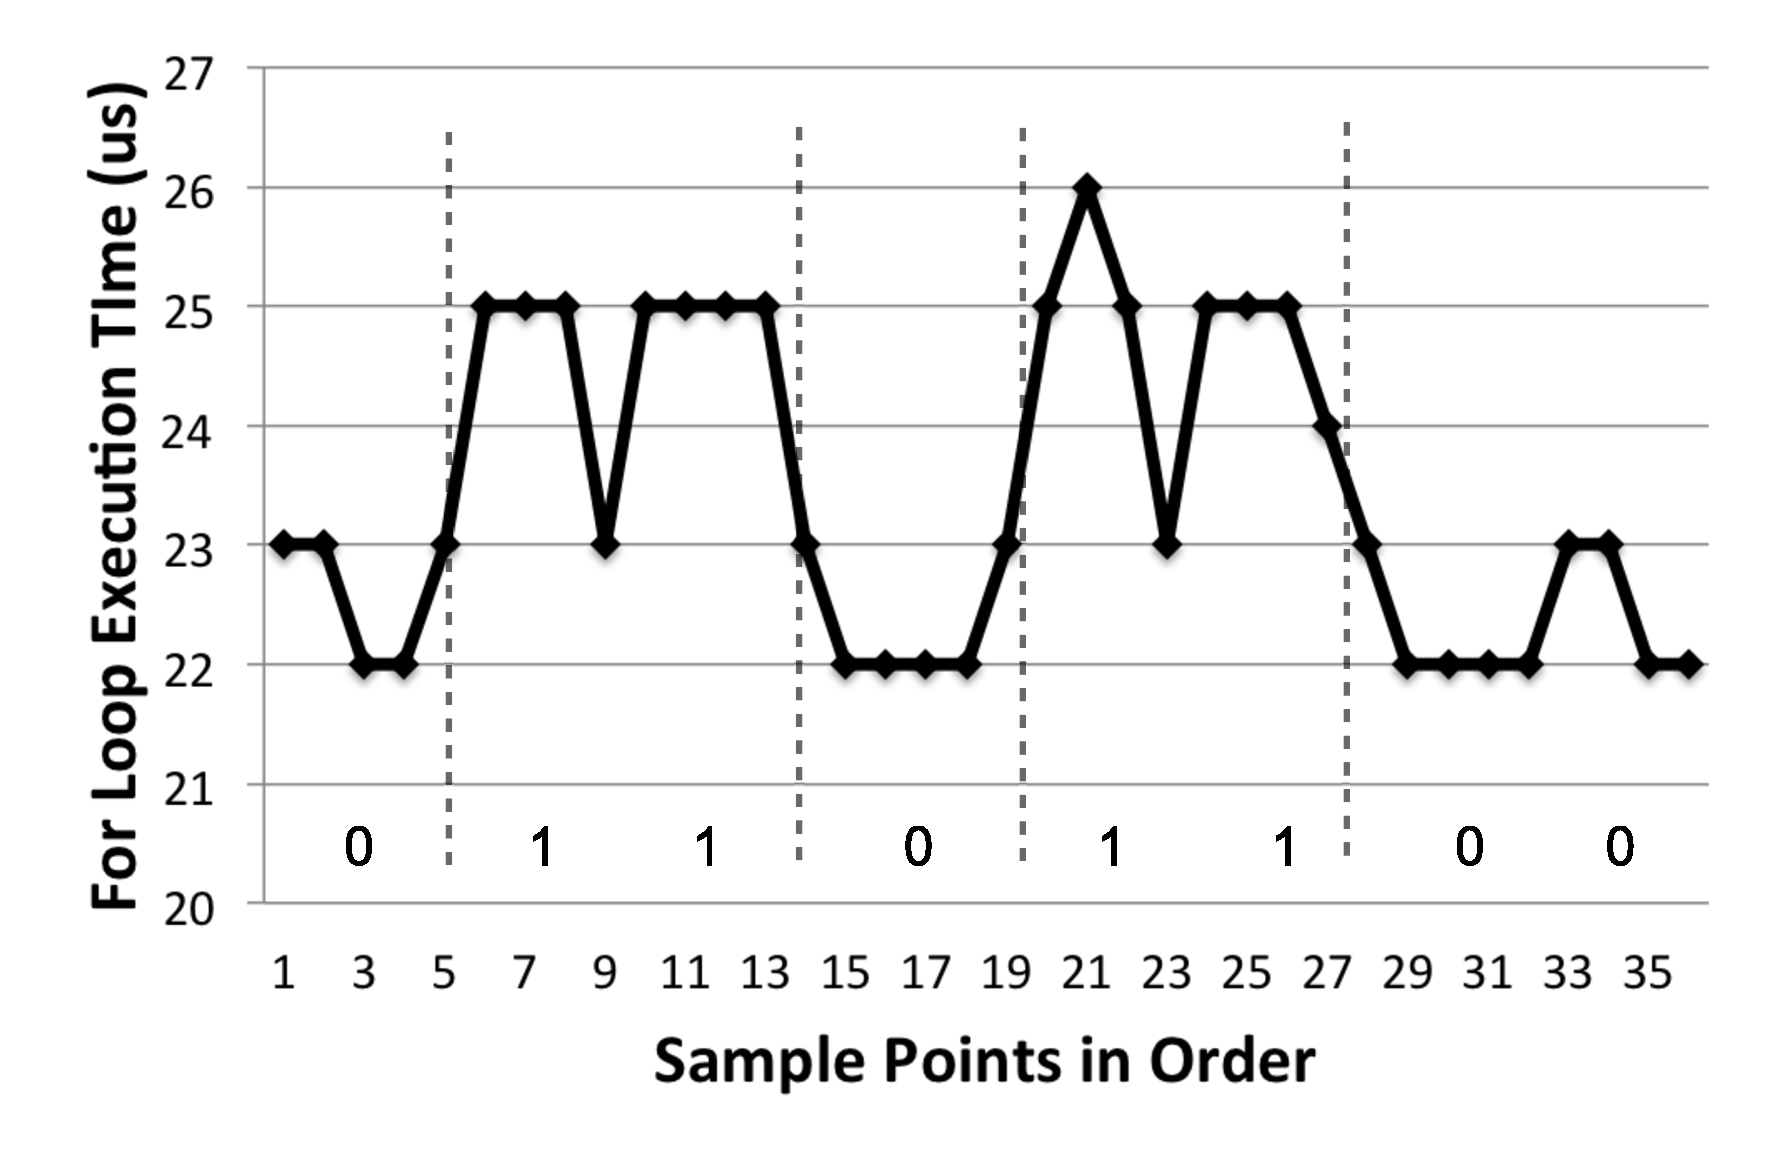
\includegraphics[width=2.79in]{figs/coherence_interference.eps}
        \caption{Attacker0's Timing Observation}
        \label{fig:coherence_interference}
    \end{center}
\end{figure}

Note that in this example, we have all the aforementioned protection schemes implemented except for the snooping bus.
Figure~\ref{fig:coherence_interference} shows the $for$ loop execution time sequence that Attacker0 observes. Each
sample point represents the time it takes to finish a 4000 iteration $for$ loop. Based on the observation, Attacker0
can recover the secret successfully. The timing variation is caused by the interference on the snooping bus. If Attacker1
produces a lot of coherent traffic, Attacker0's coherent traffic gets delayed and thus finishes slower compared to
when Attacker1 does not produce coherent traffic. 

The mechanism to protect against cache coherence timing channels consists of two parts. The first part solves the 
interference on the snooping bus. The snooping bus uses TDM to schedule the snooping requests from different timing
compartments. Each snooping request is attached with a TCID and it can only be sent during its own TC's bus turns.
This protection is the same with what we used for on-chip interconnect. 

The second part deals
with the shared data. Since the shared data is read-only, the cache miss does not necessarily have to be served by
the cache that has the Owned copy. Instead, the cache miss can always be served by the next level of cache or memory.
In our mechanism, when the cache receives a snooping request, it will first check if the TCID of the request matches its
own TCID. If the TCIDs mismatch, then the cache ignores the snooping request even if it has the data, effectively acting
as if the data does not exist. Then the cache miss will be served by the next level of cache. A tricky thing here is
coordinating the operations of multiple level of caches. In some protocols (e.g MOESI), the cache that has the Owned copy
is responsible for responding to the snooping request, so the next level of cache does not respond. In this case, the
cache needs to notify the next level of cache to respond to the snooping request. The notification message should
have a TCID that's the same with the requses so that it does not interfere with its own snooping requests on the snooping 
bus. With our design, the cache that sends a snooping request does not know the data exists on the other cache, while
the timing of the other cache's own operations is not affected.
 
\subsection{Private Per-Core Resources}

The resources that are dedicated to each core such as private caches,
TLBs, and branch predictors, are only used by one timing compartment at a time.
However, multiple timing compartments can use these resources through 
time-sharing. Therefore, there exist state-based timing channels if the state is
kept across context switches. For example, the number of cache blocks that
are evicted by one compartment may affect the number of cache hits for
another compartment in the following time slice.
We eliminate these timing channels by flushing the per-core resource state 
on a context switch that moves to a different timing compartment.
This is handled in software by the timing compartment 
manager (see Section~\ref{sec:integration_tcm}).

\subsection{Other System Resources}

Talk about DMA, I/O, etc. Managed by SW.

%\section{Protection Management}

The hardware protection mechanisms in the previous section provide tools
to implement timing compartments on a full processor. Yet, they need to be
configured and managed in software. 
%Disparate hardware timing channel protection mechanisms are not enough to 
%implement a full, timing channel secure system. It requires support from 
%software to manage the interaction of software entities with the hardware.  
%Further, these hardware mechanisms are often interdependent. The shared cache 
%miss path involves the cache, bus, and memory controller, all of which require 
%timing channel protection. Haphazardly time multiplexing these resources can 
%lead to unnecessarily large performance penalties. The integrated system 
%requires carefully coordinating the protected resources. The rest of this 
This section describes the timing compartment manager, 
%trusted software that initializes and manages timing compartments, 
and discuss how the time slices for multiple TDM mechanisms should be
coordinated together for efficiency.

\subsection{Timing Compartment Manager}
\label{sec:integration_tcm}

The timing compartment manager (TCM) is a trusted software module that is
responsible for realizing the timing compartment abstraction using the
hardware protection mechanisms.
Here, we describe TCM separately from the rest of the system.
However, in practice, TCM will be implemented as a part of the trusted software
layer such as an OS or a hypervisor.

The following discussion focuses on the interaction between the TCM and the 
hardware
protection mechanisms. In that sense, we will assume that the TCM already has
a list of timing compartments and a list of software modules such as virtual
machines and processes that belong to each timing compartment. 

%The TCM is implemented as an extension of the trusted software layer, such as 
%the OS or hypervisor. It requires functions to handle the initialization
%and context switching. It also requires a small address space of its own to 
%store the register contents of inactive TCs and a queue of inactive TCs.
%The rest of this section describes the hardware TCID storage elemnts 
%controlled by the TCM, and then elaborates on how the TCM initializes the 
%system and handles context switching.

%At system initialization time it informs the hardware of the timing 
%compartments present in the system and configures the hardware components with 
%the policy. At run time, the TCM tags requests for shared hardware resources 
%with the timing compartment ID (TCID) of the TC that originated the request.  
%Shared hardware resources then enforce the policy by checking the TCID before 
%handling the request. The hardware allows software entities within the same 
%compartment to share resources normally, and timing compartments can even be 
%allocated multiple cores.

%\begin{figure}
%    \begin{center}
%        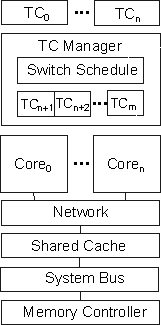
\includegraphics[width=1.08in]{figs/hw_sw_arch.pdf}
%        \caption{The Timing Compartments Architecture}
%        \label{fig:arch}
%    \end{center}
%\end{figure}

%As shown in Figure \ref{fig:arch}, the timing compartments architecture is 
%comprised of a set of $n$ cores which share resources. There is no limitation 
%on $m$, the number of timing compartments that can reside in the system at one 
%time. However, at most $n$ timing compartments can be active (executing on one 
%or more physical cores) at a time. If $m>n$, active timing compartments must 
%occasionally be switched with inactive ones. The TCM addresses this by context 
%switching TCs according to a context switch schedule.

\subsubsection{Hardware Control Interfaces}

%The hardware protection mechanisms in the previous section need to distinguish 
%memory accesses from different timing compartments.

%\subsubsection{TCIDs}

The hardware protection mechanisms track which timing compartment originated 
each request and handle the requests accordingly. Each core has a register that 
stores the TCID of the TC currently active on that core. This is used to derive 
the tags that are appended to requests originating from that core. The TCID is 
$log\ n$ bits. 

To track requests (such as network packets or shared cache accesses), they are 
tagged with a timing compartment ID (TCID). The set partitioned cache has $n$ 
registers which store the TCIDs that own each of the (at most) $n$ partitions.
When a request requires a replacement, the cache uses the TCID of the request
to decide which partitions can allow entries to be replaced according to the
policy. (Checking is only required on replacements since TCIDs have separate
address spaces.) Since the address space is partitioned, the index function can 
use the TCID as a bit mask that selects the most significant bits of the 
address. This imposes some limitations on partitioning, namely, the TCM cannot 
allocate two non-consecutive sets to a TC, and the number of sets granted to 
each TC must be a power of 2.

Each of the separate MSHR queues are tagged with a TCID of the owner, and 
requests can only affect the MSHR queues with the same TCID as the request. 
Each of the time multiplexed resources (the networks, the memory controller, 
shared cache response ports, and memory controller response ports) have $n$ 
queues.  Each of these queues has a register to store the TCID which owns that 
particular queue. A time quantum is scheduled for each queue, so time quanta 
are allocated to TCs by setting the queue configuration register with the TCID 
of that TC. A single TC can be granted multiple queues, and therefore, multiple 
time quanta in each rotation of the schedule. The configuration registers also 
control the ordering of the queues in the schedule and the time offset of the 
schedule. The offset delays the start of the schedule by some number of cycles 
to allow the TDM schedules of multiple devices to be coordinated as described 
in Section \ref{sec:coordination}. The configuration register can also set the 
duration of the time quanta for each queue, but this cannot be changed based on 
the dynamic behavior of the timing compartment.
Table~\ref{table:tcid} summarizes the TCID storage elements in the system.


\begin{table}
\begin{center}
    \begin{footnotesize}
\begin{tabular}{l|l}
    \hline
    Component & TCID Storage \\
    \hline
    Core & $n$ cores. TCID register per core. \\
    \hline
    \multirow{3}{*}{Cache}
    & $n$ response port queues. TCID register per queue \\
    & $n$ partition owner registers. \\
    & $n$ MSHR queues. TCID per queue\\
    \hline
    Network & $n$ queues. TCID register per queue\\
    \hline
    \multirow{2}{*}{Memory Controller}
    & $n$ queues. TCID register per queue \\
    & $n$ response port queues. TCID register per queue\\
    \hline
\end{tabular}
    \end{footnotesize}
    \caption{TCID storage for TC Architecture Components}
    \label{table:tcid}
\end{center}
\end{table}

%\subsubsection{Initialization \& Handling Context Switches}
%The TCM, initializes the system by setting the TCID storage elements listed in 
%Table 1 with the IDs of the initially active timing compartments. At most $n$ 
%of these can be active initially, so if $m>n$, some will be inactive, and the 
%TCM must define a static context switching schedule at initialization time.

\subsubsection{Context Switches}

% The time between context switches cannot depend on the dynamic behaviour of 
% the TCs. Otherwise, a timing compartment could observe the time that they are 
% context switched in or out to learn information about the timing compartment 
% it is switched with. Instead, context switches occur at a fixed time 
% interval, $T_{CTX}$. Every $T_{CTX}$ cycles the TCM is invoked to replace the 
% timing compartment which has been active the longest with the TC at the head 
% of the inactive TC queue. The compartment which has been switched out is 
% moved to the back of the inactive TC queue.

Although private, per-core resources are not concurrently shared by TCs, they 
are shared across context switches. The state modified by the TC that is 
swapped out can affect the timing of the TC that is swapped in.
To perform the context switch, the CPU pipeline and the memory request queue 
are drained. The general purpose registers of the outgoing TC are stored in 
TCM-space memory and tagged with the TCID. The private cache, shared cache 
partition, TLB, and branch predictor state of the outgoing TC are all flushed.  
Finally, the TCID stores of the outgoing TC are replaced with the TCID of the 
incoming TC. 

The time required to perform a context switch depends on the state and behavior 
of the outgoing TC. The owner of the incoming TC can observe when the incoming 
TC begins executing, so this implies a potential leakage of secrets.  To 
prevent this, context switches are bound to always take the worst case time.  
If a context switch completes early, the incoming TC is stalled until the worst 
case context switch time has been reached.

\subsection{Time Slice Coordination}
\label{sec:coordination}
Naïvely time multiplexing the components with contention based timing channels 
can lead to poor performance since many of these components are on the same 
path to handle a request. 
% During a shared cache miss, the request is sent along the bus that connects 
% the private caches to the shared cache, which we refer to as the L2L3Bus.  
% After detecting the miss, a request is sent to memory through the bus 
% connecting the shared cache to the memory controller, which we refer to as 
% the membus. The memory controller handles the memory request and sends the 
% response back through the membus. Finally, the cache sends a response back 
% through the L2L3Bus.
%%%%%%% The NoC section should mention the request/response layers before this 
%%%%%%% section
On the cache miss path both buses (which are each split into a request and 
response layer), the response ports of the cache and memory controller, and the 
memory controller itself are all time multiplexed. A naïve system design might 
determine an optimal time quantum duration and round robin schedule for each 
resource independently of one another as shown in figure 
\ref{fig:naive_scheme}. The L2-L3 bus is the bus connecting the private caches 
to the shared cache, and the membus connects the shared cache to the memory 
controller.

\begin{figure}
    \begin{center}
        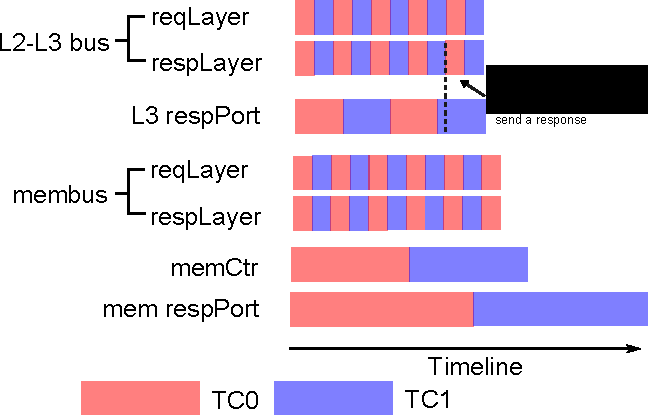
\includegraphics[width=3.46in]{figs/baseline_schedule.pdf}
        \caption{Cache hit timing sequence.}
        \label{fig:naive_scheme}
    \end{center}
\end{figure}

Notably, the time quanta of each component are not aligned with each of the 
L2-L3 bus time quanta.  During a shared cache hit on behalf of $TC1$, 
occasionally the $TC1$ shared cache response port time quantum will be aligned 
with the $TC1$ L2-L3 bus time quantum allowing it to proceed along the path 
without unneeded stalls.  However, sometimes these are not well-aligned and 
$TC1$ will have to wait for $TC2$ to finish before it can proceed. This becomes 
even more wasteful
as the number of timing compartments scales. A request may have to wait through 
each other compartment's time quantum. 

\begin{figure}
    \begin{center}
        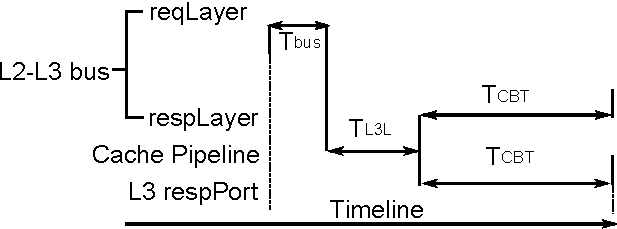
\includegraphics[width=2.4675in]{figs/hit_timing.pdf}
        \caption{Cache hit timing sequence.}
        \label{fig:hit_timing}
    \end{center}
\end{figure}

For ease of analysis, we examine the shared cache hit path before covering the 
complete shared cache miss path. Figure \ref{fig:hit_timing} shows the timing 
of $N$ requests through the shared cache hit path, where $N$ is the number of 
pipeline stages through the fully pipelined cache. Sending a request over the 
L2-L3 bus takes $T_{bus}$ cycles.  The cache then takes $T_{L3L}$ cycles after 
receiving the request before the data for the first of the $N$ requests is 
available to be sent. The response port transfers all the responses in $N\times 
T_{CBT}$ cycles, where $T_{CBT}$ is the time required to transfer a cache block 
over the bus. $T_{hit}$, the total period of the the cache hit timing sequence 
is $T_{bus}+T_{L3L}+N\times T_{CBT}$.

\begin{figure}
    \begin{center}
        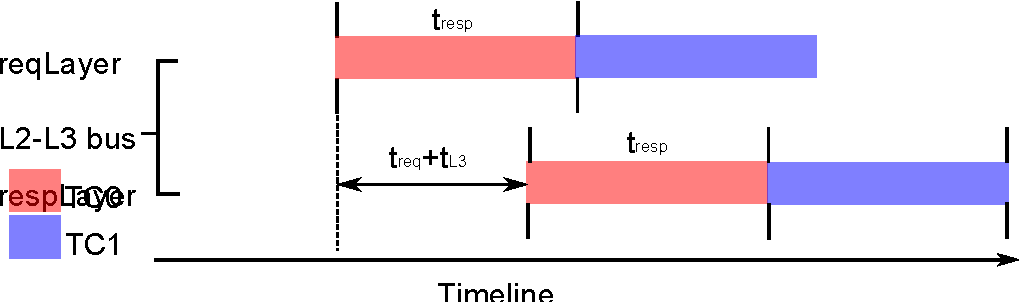
\includegraphics[width=3.2624in]{figs/hit_schedule.pdf}
        \caption{Cache hit timing path schedule.}
        \label{fig:hit_schedule}
    \end{center}
\end{figure}

To improve over the naïve scheme, the schedule must coordinate each of these 
resources to 1) allow a request to proceed through common paths unblocked and 
2) repeat this alignment for each TC. Figure \ref{fig:hit_schedule} shows a 
schedule that allows $N$ requests to proceed unblocked for each TCs turn. The 
time quanta are aligned to follow the timings of \ref{fig:hit_timing}. To 
guarantee that the behavior of a schedule repeats for the time quanta of each 
TC, the durations of the time quanta for each resource must share a common 
factor number of cycles. For example, if $N \times T_{CBT}$ (and this is the 
time quanta duration for the response port and layer) is 16 and $T_{bus}$ is 3, 
the actual time quanta duration for the request layer, $T_{req}$, should be 4, 
8, or 16 even though the request port cannot do useful work for these extra 
cycles. 

\begin{figure}
    \begin{center}
        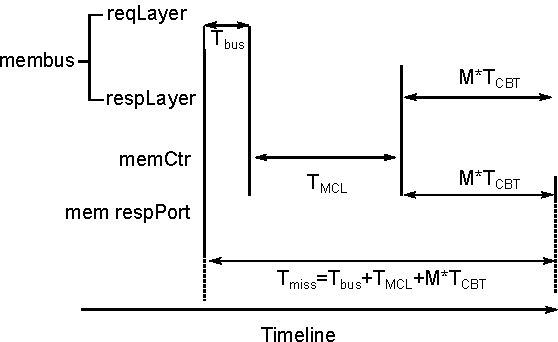
\includegraphics[width=2.9475in]{figs/miss_timing.pdf}
        \caption{The shared cache miss path timing sequence.}
        \label{fig:miss_timing}
    \end{center}
\end{figure}

The analysis for the segment of the shared cache miss path between the shared 
cache and the memory controller is similar. The most significant difference is 
that unlike the cache, the memory controller itself is time multiplexed. Figure 
\ref{fig:miss_timing} shows the timing for this segment of the shared cache 
miss path. The time quanta of the memory controller have a duration that is 
chosen to be $T_{MCL}$. This optimal value may depend on the design, and
the authors of \cite{ushpca14} discuss the selection of this value. $M$ is the 
number of memory requests that can be handled in a single memory controller 
time quantum.
$T_{miss}$, the total period of the cache miss timing sequence is 
$T_{bus}+T_{MCL}+M\times T_{CBT}$.

The schedule of the entire system should allow the shared cache miss path to be 
traversed unblocked.
% , but since cache hits are more frequent than misses, the performance of the 
% cache hit path should not be weakened to meet this goal.
To prevent blocking along the request path, the time quantum of a timing 
compartment on the membus request port should begin just as that timing 
compartment's time quantum on the shared cache memory side request port 
finishes. This prevents blocking along the request path of the membus.
Similarly, to prevent blocking along the response path, the time quantum of the 
shared cache response port should begin just after the time quantum of the same 
timing compartment on the memory bus response layer ends. Figure 
\ref{fig:coordination}
shows a high level view of a full coordinated schedule.

\begin{figure}
    \begin{center}
        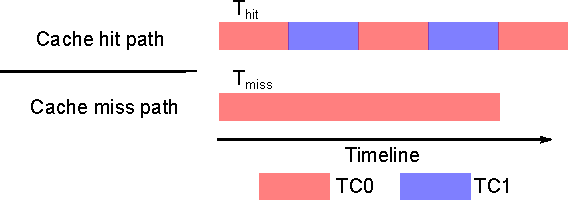
\includegraphics[width=2.9475in]{figs/coordination.pdf}
        \caption{A coordinated cache miss path schedule.}
        \label{fig:coordination}
    \end{center}
\end{figure}

To meet the first criterion, the cache hit path timing sequence shown in 
\ref{fig:hit_timing} should be aligned with the start of the corresponding 
memory bus time quantum. To repeat this behavior for each cache hit path timing 
sequence, $T_{hit}$ and $T_{miss}$
should share a common factor. Since cache hits are more frequent than misses, 
the performance of the cache hit path should not be weakened to accomplish 
this. Instead, the length of the membus timing sequence should be increased 
(e.g. by increasing the memory controller time quantum). The second criterion 
is met if the maximum number of active timing compartments in the system (i.e.  
the number of cores) is a factor of the period of the membus timing sequence.

%\section{Cache Coherence Timing Channel}
In a multi-core system, threads are running concurrently on different cores. These threads may share some
data which they read from or write to. The shared data thus can have multiple copies exist in each core's
private cache. In general, a cache coherence protocol is used to ensure each thread gets the most updated
data to work with.

In a snooping-based protocol, the caches on the same level are connected with a snooping bus. When a request
comes into a cache and incurs a cache miss, a snooping request is sent on the snooping bus. All the other
caches observe the snooping request, and one of them may respond to the request by forwarding the data if 
the data exists. The operations to handle snooping requests and responses highly depend on the specific cache 
coherence protocols being used. Commonly used protocols include MSI, MESI and MOESI~\cite{mark_book}.

If different timing compartments share data, there is clearly a timing channel introduced by the cache coherence
protocols. For example, TC0 wants to write to A, and A exists in TC1's cache. In order to perform the write, the
cache coherence protocol will invalidate A in TC1's cache. Later when TC1 wants to read A, it will incur a cache
miss which indicates TC0 has written to A. In our threat model, we assume timing compartments do not share data. 
So the above mentioned timing channel is not a concern. However, our assumption only guarantees the cache state
is not affected by cache coherence protocols. The snooping bus is shared by different timing compartments, thus 
the coherent traffic can still interfere with each other. The interference on the snooping bus introduces timing
channel, as shown in the example below.

\subsection{Covert Channel Attack Example}
In this section, we demonstrate a covert channel attack example on a four-core system. The system configuration 
is shown in Figure~\ref{fig:coherent_system}. Each core has a private L1 and L2 cache, and the four cores share
the L3 cache. The four L2 caches are connected with a snooping bus which uses a MOESI protocol. 
In this example, there are two attackers who
want to communicate a secret data when the direct communication between them is strictly disallowed. Each attacker 
belongs to a different timing compartment. Attacker0 occupies core 0 and core 1 while attacker1 occupies core 2 and
core 3. 

\begin{figure}
    \begin{center}
        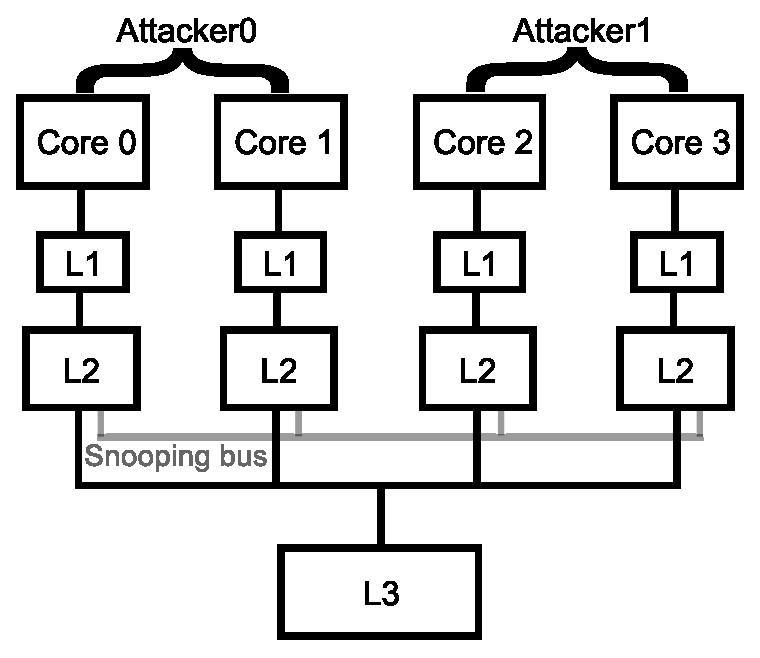
\includegraphics[width=2.3in]{figs/coherent_system.eps}
        \caption{System Configuration}
        \label{fig:coherent_system}
    \end{center}
\end{figure}

Attacker0 has two threads, each running on a different core. Both threads run a $for$ loop of 4000 iterations, and
write to a shared data in each iteration. Before each write is performed, one L2 cache has to forward the data
to the other L2 cache through the snooping bus and invalidates its own copy, according to the cache coherence protocol. 
As a result, there is a lot of coherent traffic between these two threads. Attacker0 runs this $for$ loop repeatedly and
records the time to finish the $for$ loop using c++ timing functions.

Attacker1 owns the secret data ('01101100') and tries to communicate this secret to Attacker0. It checks each bit
in the secret data. If the bit is 0, it executes a $for$ loop which writes to a data in each iteration. This does not produce 
coherent traffic. If the bit is 1, Attacker1 spawns a new thread, which also runs a $for$ loop that writes to the same data, hence producing a lot of coherent traffic. 

\begin{figure}
    \begin{center}
        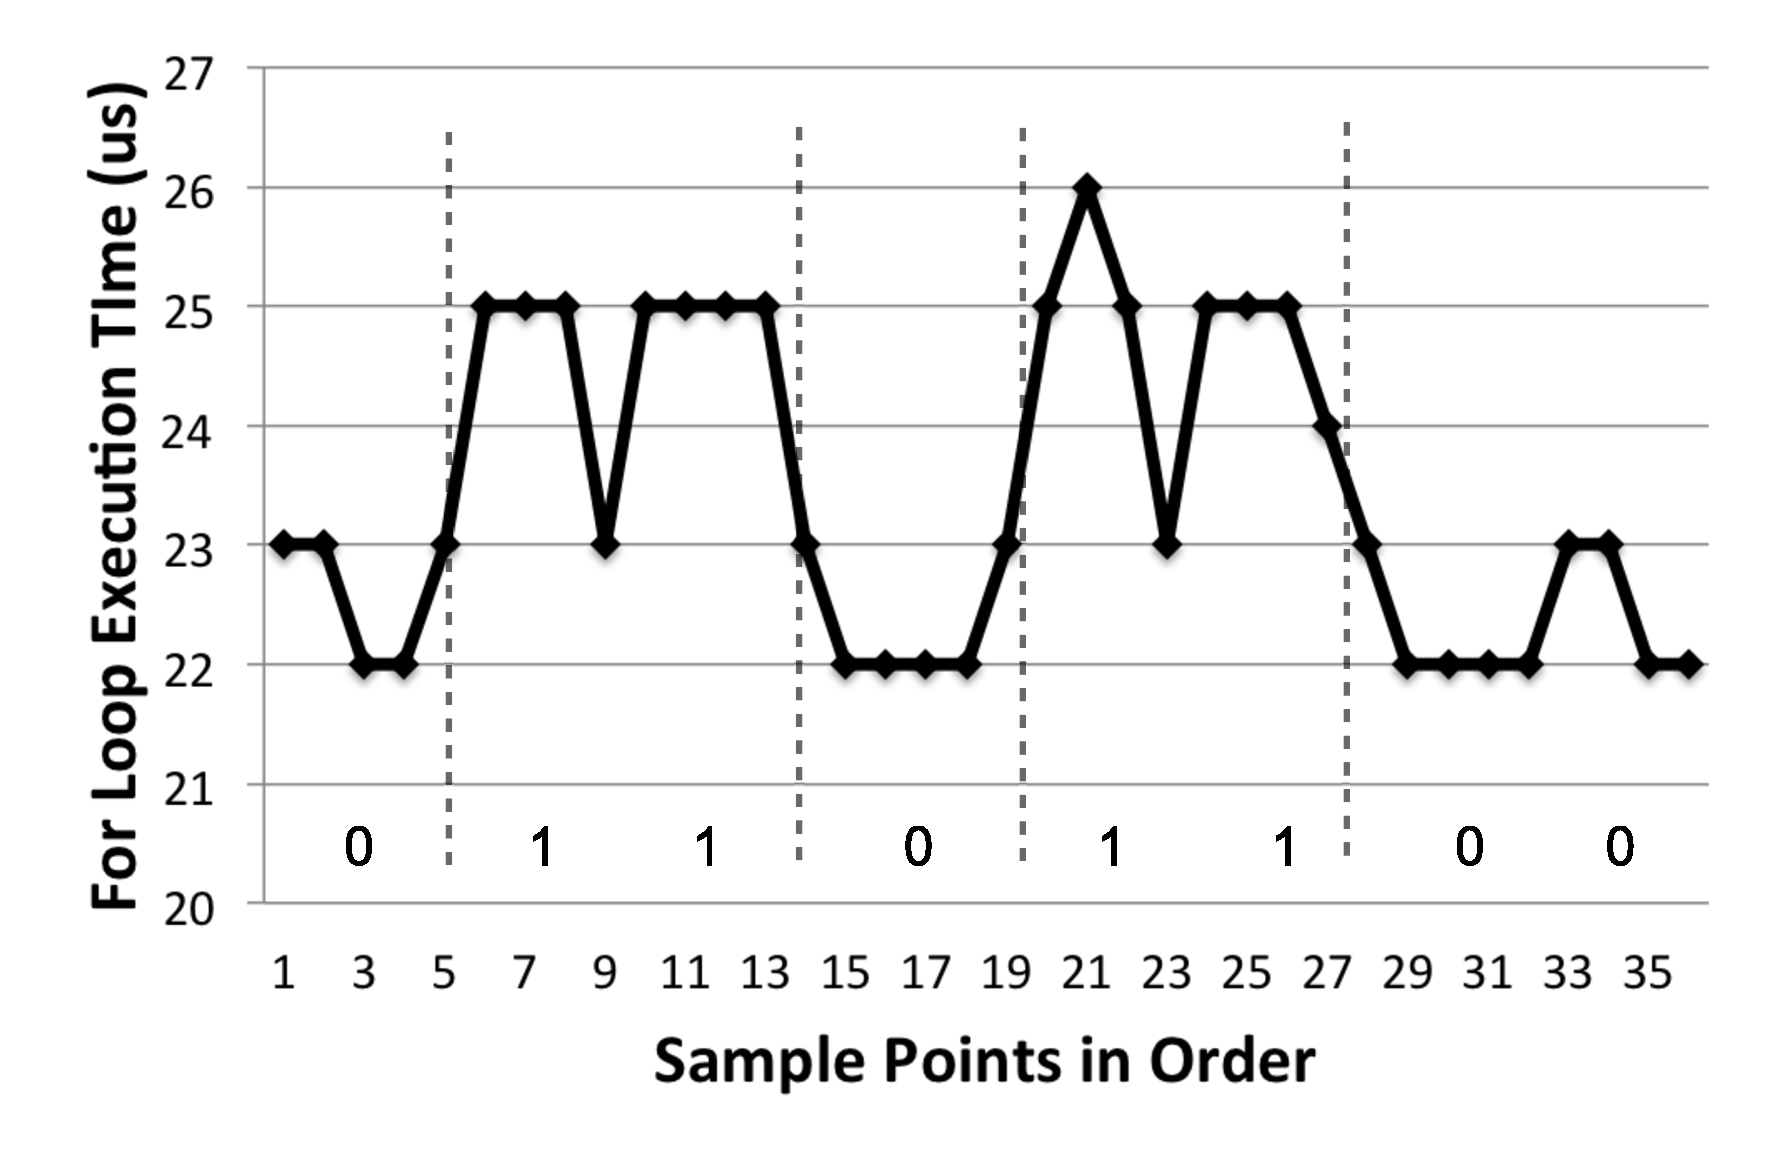
\includegraphics[width=2.79in]{figs/coherence_interference.eps}
        \caption{Attacker0's Timing Observation}
        \label{fig:coherence_interference}
    \end{center}
\end{figure}

Note that in this example, we have all the aforementioned protection schemes implemented except for the snooping bus.
Figure~\ref{fig:coherence_interference} shows the $for$ loop execution time sequence that Attacker0 observes. Each
sample point represents the time it takes to finish a 4000 iteration $for$ loop. Based on the observation, Attacker0
can recover the secret successfully. The timing variation is caused by the interference on the snooping bus. If Attacker1
produces a lot of coherent traffic, Attacker0's coherent traffic gets delayed and thus finishes slower compared to
when Attacker1 does not produce coherent traffic. 

\subsection{Protection Scheme}
The protection scheme is similar to the normal bus protection. We attached the TCID to the snooping requests and responses.
The snooping bus scheduling is changed to round-robin scheduling. With this protection, the coherent traffic from different
timing compartments do not interfere with each other through the snooping bus. This protection prevents the covert channel
attack mentioned above.

%%%%%%%%%%%%%%%%%%%%%%%%%%%%%%%%%%%%%%%%%%%%%%%%%%%%%%%%%%%%%%%%%%%%%%%%%%%%%%%
%% Outline
%%%%%%%%%%%%%%%%%%%%%%%%%%%%%%%%%%%%%%%%%%%%%%%%%%%%%%%%%%%%%%%%%%%%%%%%%%%%%%%
% 
% Explain problem without timing details. Use figure that has turn lengths with 
% no offsets. Show a packet traversing through path with latencies outlined and 
% the packet getting delayed. Explain figure.
% 
% Though the l3 hit path is simple, whole l2 miss path is a nontrivial problem 
% - many tradeoffs, used linear optimization. Wrote simulator to explore this.  
%   Ultimately found a general scheme
% that an optimizer couldn't beat for the l3 miss path. Finding agood balance 
% between
% the hit and miss paths required an optimizer and we did not find a general 
% scheme
% 
% \subsection{L2 Miss Timing Sequence}
% Introduce l3 hit timing sequence with figure. Explain figure.
% 
% Show l3 miss timing sequence. Use figure.
% 
% \subsection{Latency Simulator \& Optimal Coordination}
% 
% Explain goal of coordinating (EV of L2 miss latency). Usually achieved by 
% aligning turns of adjacent devices. Use turn lengths (duration a TC is 
% scheduled to use a device - depends time to send message, affects 
% ``randomness'' of schedule) and offsets (difference in start times that
% improves how the schedule relates to the schedule of other devices).
% 
% Show how to optimize l3 hits. Use figure.
% 
% Explain tradeoffs. Use figure?? It is not simple to solve.
% 
% Wrote our own l2 miss (l2 to l2) timing simulator. Explain what it simulates.  
% (Assumes uniform random arrival, calculate latency for every possible arrival 
% in a schedule, gets EV of latency).
% 
% Exhaustive search of L3 hit path. Confirms that an intuitive design is best.
% 
% Cannot exhaustively search L3 miss path latencies. Instead use linear 
% optimizatin. Search space has many relative minima (change offset slightly, 
% suddenly schedule is much better) - cannot use hill climbing. Use simulated 
% annealing. Explain our simulated annealing implementation. Optimize for l3 
% miss alone and l2 miss latency assuming hit rate of 90\%.
% 
% Tried a scheme we suspected would have a good L3 miss latency. Optimal result 
% was different. Adjusted optimizer result to something that made more 
% intuitive sense and iterated. Reran optimizer on result of iterative 
% approach, and the optimizer could not find a better scheme in 20,000 steps.
% 
% Explain optimal scheme. Use figure.
% 
% For l2 miss latency, no intuitive general approach could be found. Balance 
% between hit/miss paths is difficult.


%%%%%%%%%%%%%%%%%%%%%%%%%%%%%%%%%%%%%%%%%%%%%%%%%%%%%%%%%%%%%%%%%%%%%%%%%%%%%%%
%% Old Figures
%%%%%%%%%%%%%%%%%%%%%%%%%%%%%%%%%%%%%%%%%%%%%%%%%%%%%%%%%%%%%%%%%%%%%%%%%%%%%%%
% \begin{figure}
%     \begin{center}
%         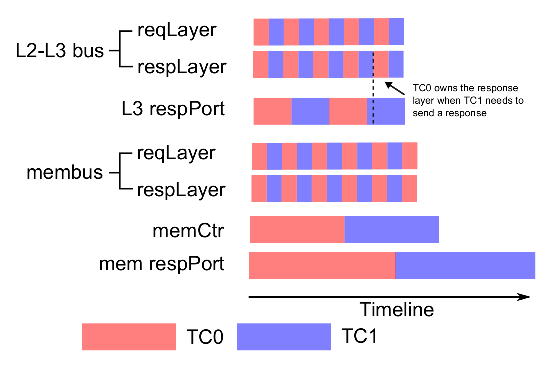
\includegraphics[width=3.46in]{figs/baseline_schedule.eps}
%         \caption{Cache hit timing sequence.}
%         \label{fig:naive_scheme}
%     \end{center}
% \end{figure}
% 
% 
% \begin{figure}
%     \begin{center}
%         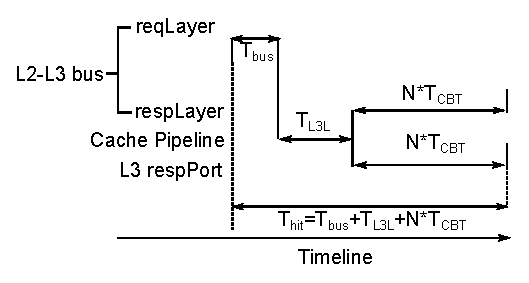
\includegraphics[width=2.4675in]{figs/hit_timing.eps}
%         \caption{L3 cache hit timing sequence.}
%         \label{fig:hit_timing}
%     \end{center}
% \end{figure}
% 
% \begin{figure}
%     \begin{center}
%         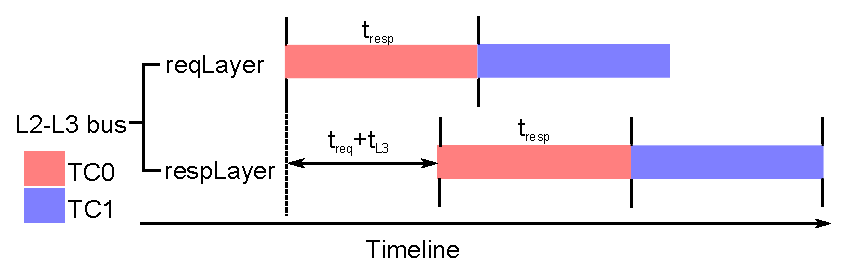
\includegraphics[width=3.2624in]{figs/hit_schedule.eps}
%         \caption{Cache hit timing path schedule.}
%         \label{fig:hit_schedule}
%     \end{center}
% \end{figure}
% 
% \begin{figure}
%     \begin{center}
%         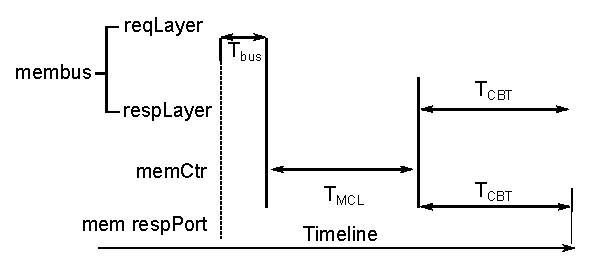
\includegraphics[width=2.9475in]{figs/miss_timing.eps}
%         \caption{The L3-memory timing sequence.}
%         \label{fig:miss_timing}
%     \end{center}
% \end{figure}
% 
% \begin{figure}
%     \begin{center}
%         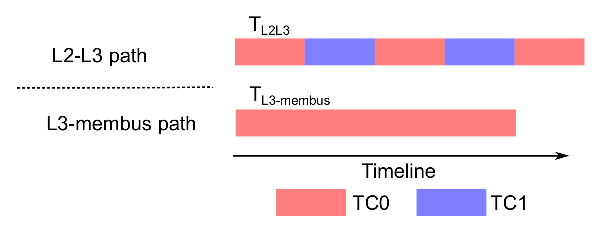
\includegraphics[width=2.9475in]{figs/coordination.eps}
%         \caption{A coordinated cache miss path schedule.}
%         \label{fig:coordination}
%     \end{center}
% \end{figure}

\section{Time Slice Coordination}
\label{sec:coordination}
The Timing Compartments architecture relies heavily on time multiplexing to 
protect shared resources including the L2-L3 bus, the L3-memory bus, and the 
memory controller. These resources frequently interact since each is involved 
in handling L2 misses. If the time multiplexing schedules for each of these 
resources are not designed to account for this interaction, it could lead to 
exorbitant latencies and wasted bandwidth.

\begin{figure}
    \begin{center}
        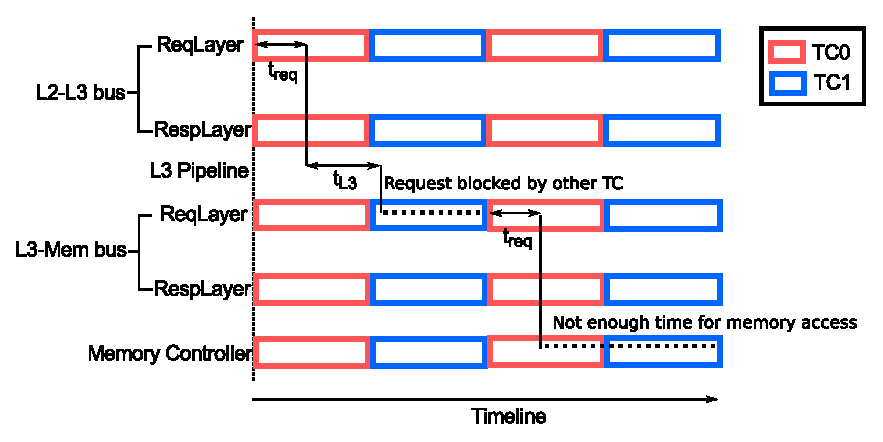
\includegraphics[width=3.0in]{figs/problem.eps}
        \caption{A poorly performing time multiplexing schedule.}
        \label{fig:problem}
    \end{center}
\end{figure}

Figure \ref{fig:problem}, illustrates the problem. It shows when each of two 
timing compartments are scheduled to use the time multiplexed resources along 
the L2 miss path. Green blocks indicate that TC0 is scheduled to use the device, 
and blue blocks indicate that TC1 is scheduled. We refer to the block of time 
that a timing compartment is scheduled to use a device as the \emph{turn} and 
we refer to the duration of a turn as the \emph{turn length}. In this schedule, 
timing compartments are allotted the same turn length for each time multiplexed 
resource, and the schedule for each device starts at the same time.

%%%%%%%%%%%%%%%%%%%%%%%%%%%%%%%%%%%%%%%%%%%%%%%%%%%%%%%%%%%%%%%%%%%%%%%%%%%%%%%
%% This section is easier to write if we introduce bus layers in the uarch 
%% channel section (section 3)
%%%%%%%%%%%%%%%%%%%%%%%%%%%%%%%%%%%%%%%%%%%%%%%%%%%%%%%%%%%%%%%%%%%%%%%%%%%%%%%
An L3 miss from TC0 is shown proceeding with these time multiplexing schedules.
The miss begins at the L2 request layer where the request is sent to the L3.  
When the L3 access is complete, the request must proceed through the L3-memory 
bus request layer, but at this time TC1 is scheduled to use the L3-memory 
request layer, so it must wait for TC1's turn to finish before the request can 
proceed to the memory controller. Then, when it arrives at the memory 
controller, there is not enough time left in the turn to complete a request, so 
it is blocked again. There are similar issues as the packet traverses the rest
of the path.

Clearly, this schedule is inefficient. When designing a schedule for these 
resources both the L3 hit and L3 miss paths should be considered. In this 
section we describe the timing for both paths. We then show that devising a 
schedule that optimizes just the hit path is straightforward, but scheduling 
the miss path and balancing both is challenging.

\subsection{L2 Miss Timing Paths}
To efficiently time multiplex the resources involved in an L2 miss, 
we must understand the timing of L2 misses. L2 misses take two different 
paths and have different timings depending on whether the L2 miss is an L3 hit 
or miss. This section analyzes L2 miss timings under both cases: an L2 miss
followed by an L3 hit, and an L2 miss followed by an L3 miss.

Figure \ref{fig:hit_timing} shows the timing for an L3 hit. The arrows 
indicate the time that the resource in the corresponding column is used.
The L2 miss begins by transferring a request over the L2-L3 bus request layer 
in $t_{req}$ cycles. Typically, $t_{req}$ depends on how the bus protocol 
requires requests to be sent. The request then arrives at the L3 cache, where 
it takes $t_{L3}$ cycles (i.e. the L3 cache latency). We assume the cache is 
fully pipelined, so even if a request arrives one cycle after another, both can 
use the cache simultaneously, and the access always completes in $t_{L3}$ 
cycles. Finally, the data is transferred from the L3 response port back to the 
L2 over the L2-L3 bus response layer in $t_{resp}$ cycles. Often, $t_{resp}$ 
will be greater than $t_{req}$. It depends on the bus bandwidth and the size of 
a cache block.

\begin{figure}
    \begin{center}
        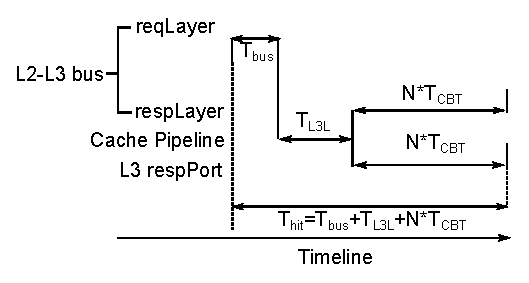
\includegraphics[width=2.5in]{figs/hit_timing.eps}
        \caption{L3 cache hit timing sequence.}
        \label{fig:hit_timing}
    \end{center}
\end{figure}

Figure \ref{fig:miss_timing} shows the timing for an L3 miss. The request 
begins by transferring over the L2-L3 bus request layer, and similarly takes 
$t_{L3}$ cycles to identify that it is a miss. Afterwards, it sends another 
request to the memory controller over the L3-memory bus request layer in 
$t_{req}$ cycles. Memory requests take variable time to complete, after which 
the data is returned to the L3 in $t_{resp}$ cycles, written to the L3 in 
$t_{L3}$ cycles and finally returned to the L2 after another $t_{resp}$ cycles.

\begin{figure}
    \begin{center}
        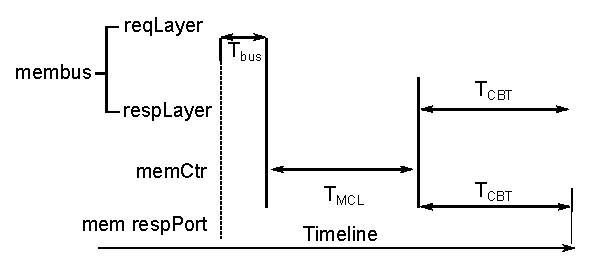
\includegraphics[width=2.8in]{figs/miss_timing.eps}
        \caption{L3 cache miss timing sequence}
        \label{fig:miss_timing}
    \end{center}
\end{figure}

\subsection{Devising a Schedule}
A good time multiplexing schedule should minimize the average L2 miss latency.
We can achieve this by controlling the turn lengths and offsets for each 
time multiplexed device. Here, an \emph{offset} refers to a shift in the start 
of the first turn for a single device compared to the start of the full 
schedule.
For a particular resource, suitable turn lengths depend on the latency of that 
resource, and suitable offsets depend on the latency of the preceding resource. 


There are three main criteria for developing an efficient schedule.
First, the turn length should be long enough for the resource's action 
to complete. Second, the offset should make sure the turn starts when the data is 
available from the preceeding device.
Third, it is desirable for the schedule to repeat in a short number of cycles.
Turns are allocated for each timing compartment in a repeated sequence
(e.g. 1,2,3,4,1,2,3,4 for four timing compartments). Therefore, a schedule
for the entire L2 miss path repeats after the least common multiple of each turn
length in the path multiplied by the number of timing compartments. Schedules 
with turn lengths that have a high least common multiple will often be erratic, 
causing the turns of each device to shift relative to one another and cause bad 
timings.

\subsubsection{L2 Misses Followed by L3 Hits}
This reasoning can be applied in a straightforward way to derive the schedule 
that optimizes the L2 miss latency assuming it is followed by an L3 hit.
The optimal schedule is shown in Figure~\ref{fig:hit_schedule}.
From the timing for this case shown in Figure~\ref{fig:hit_timing}, the turn
length for the L2-L3 request layer must be greater than $t_{req}$. The 
data is available to the L2-L3 response layer after $t_{req}+t_{L3}$ cycles, so 
this is used as the offset for the response layer. The turn length for the 
response layer is $t_{resp}$. Since typically $t_{req}<t_{res}$ we could use a 
shorter turn length for the request layer. However, any requests from one TC 
would be queued until the turn for the same TC on the response layer starts, so 
this provides no benefit. In fact, reducing the turn length causes requests 
that arrive later in the schedule to incur extra delays. Finally, since the 
turn lengths for both the request and response layers are the same, the 
schedule repeats frequently as desired. The schedule parameters are summarized 
in the top of Table~\ref{tab:l2_miss_schedules}.

\begin{figure}
    \begin{center}
        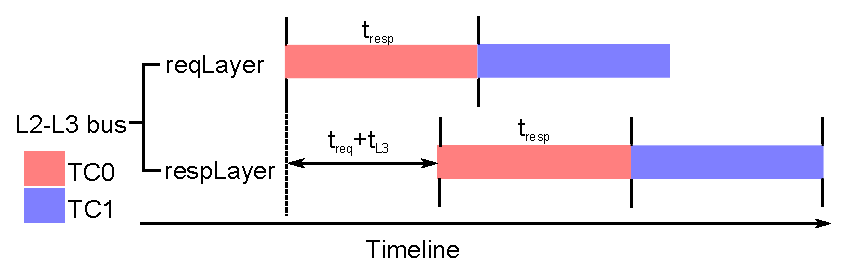
\includegraphics[width=2.5in]{figs/hit_schedule.eps}
        \caption{Cache hit timing path schedule.}
        \label{fig:hit_schedule}
    \end{center}
\end{figure}

\subsubsection{L2 Misses Followed by L3 Hits}
Deriving a schedule that is suitable for L2 misses assuming they are followed 
by L3 misses is similar. The turn lengths for both L3-memory bus layers and
the memory controller should be $t_{mem}$, the minimum memory turn length.
Although these bus turns could have been smaller, this would provide no
benefit since they transfer responsesto and from the memory controller exclusively.
The L2-L3 bus layer turn lengths should be
the smallest factor of $t_{mem}$ greater than $t_{resp}$. The L2-L3 bus turn 
lengths are greater than just $t_{resp}$ to improve the schedule's repeatability.
Each device schedule is offset so that it starts when the data is available 
based on the timing of an L2 miss followed by an L3 miss shown 
in~\ref{fig:hit_timing}. Table \ref{tab:l2_miss_schedules} summarizes both the
turn lengths and offsets in this schedule. Here $t_{read}$ is the worst case
memory read time and
\[
  t_{req}^+ = Min(\{n | \exists m\in \mathbb{N}.t_{mem}=m\cdot n, n > t_{resp}\})
\]
As discussed in Section~\ref{sec:eval_coord} we did not find a schedule with 
a lower average L2 miss latency given that it is followed by an L3 miss.

\def\dc{Blue}
\begin{table}
    \caption{Efficient L2 miss schedules by case.}
    \centering
    \begin{tabular}{|r|r|l|l|}
        \hline
        \multicolumn{4}{|l|}{L2 misses followed by L3 hits}\\\hline
        \multicolumn{2}{|l|}{Device Name} & Turn Length & Offset\\\hline
        \multicolumn{2}{|l|}{L2-L3 Req}  & $t_{resp}$ & 0\\\hline
        \multicolumn{2}{|l|}{L2-L3 Resp} & $t_{resp}$ &
          $t_{req}+t_{L3}$\\\hline\hline
        \multicolumn{4}{|l|}{L2 misses followed by L3 misses}\\\hline
        \multicolumn{2}{|l|}{L2-L3 Req}   & $t_{resp}^+$ & 0\\\hline
        \multicolumn{2}{|l|}{L3-Mem Req}  & $t_{mem}$ & $t_{req}+t_{L3}$\\\hline
        \multicolumn{2}{|l|}{Mem Ctl}     & $t_{mem}$ & $2t_{req}+t_{L3}$\\\hline
        \multicolumn{2}{|l|}{L3-Mem Resp} & $t_{mem}$ & 
          $2t_{req}+t_{L3}+t_{read}$\\\hline
        \multicolumn{2}{|l|}{L2-L3 Resp}  & $t_{resp}^+$ &
          $2t_{req}+2t_{L3}+t_{read}+t_{resp}$\\\hline
    \end{tabular}
    \label{tab:l2_miss_schedules}
\end{table}

\subsubsection{L2 Misses in general}
Scheduling for L2 misses in general, without assuming it is followed by a hit 
or a miss, is much more difficult. Notice that the L2-L3 request and response 
layer turn lengths and the L2-L3 response layer offsets in the efficient 
schedules for the L3 miss and L3 hit cases are different. These differences 
must be balanced for an L2 miss schedule. To ensure repeatability, it is 
unclear if it is preferable to increase the L2-L3 request layer turns to 
$t_{resp}^+$ at the expense of the more common hit case, or if it is better to 
increase the memory controller turn length possibly worsening a bottlneck.
Further, an offset that works well is highly dependant on the actual system 
parameters: $t_{L3}$, $t_{req}$, $t_{resp}$, and $t_{read}$.
We examined this scheduling problem with a simulated annealing optimizer,
and although we could not construct much meaning from the optimal 
schedule, we will show in Section \ref{sec:eval_coord} that the gap between
the best and worst schedules is significant. This suggests that although time 
multiplexing the L2 miss path is a difficult problem, it can greatly impact 
performance.

\section{Evaluation}

We evaluated the timing compartments architecture using the gem5 architectural 
simulator~\cite{gem5} integrated with the DRAMSim2~\cite{DRAMSim2} 
memory simulator. Our experiments use multiprogram workloads 
comprised of SPEC2006 benchmarks compiled for the ARM ISA. 

Table~\ref{tab:config} shows our system configuration.
The cores use the gem5 ``O3`` out-of-order core model which runs at 2GHz. 
Each core has private 32KB L1 instruction and data caches, and private 256KB L2 
cache. The cores share a 4MB L3 cache. We derived cache configuration 
parameters from the Intel Xeon E3-1220L, which is a two core architecture used 
by Amazon EC2. In DRAMSim2, we simulate a 667MHz 2GB DDR3 memory. The 
interconnects in the simulator runs at 1GHz. Unless specified otherwise, each experiment is 
fastforwarded for 1 billion instructions, and run for 100 million 
instructions. We will first describe our security evaluation and then show
the performance evaluation.

\begin{table}
    \caption{Simulator configuration parameters.}
    \centering
    \begin{tabular}{|l|l|l|r|}
        \hline
        \multicolumn{3}{|l|}{gem5 core model} & ``O3''        \\\hline
        \multicolumn{3}{|l|}{CPU Clock}    & 2GHz             \\\hline
        \hline
        \multicolumn{2}{|l|}{Memory}             & 2GB    & 667MHz  \\\hline
        \hline
        \multicolumn{3}{|l|}{Network Clock}      & 1GHz \\\hline
        \hline
        L1d / L1i  & 32kB   & 2-way  & 2 cycles\\\hline
        L2         & 256kB  & 8-way  & 7 cycles \\\hline
        L3         & 4MB    & 16-way & 17 cycles  \\\hline
    \end{tabular}
    \label{tab:config}
\end{table}

\subsection{Security Evaluation}

To experimentally evaluate the security of the timing channel protection in our 
architecture, we use a two-core system with two timing compartments, TC0 and
TC1, running concurrently. The protection policy is configured to disallow any 
timing channels between the two compartments. If the number of cycles required 
to execute a certain number of instructions for a particular benchmark running on 
TC0 depends on which benchmark is running on TC1, it indicates timing 
interference exists that can be exploited to leak information about TC0. A 
secure system should guarantee the benchmark running in TC0 always uses the 
same number of cycles to finish regardless of which benchmark TC1 is running. 

Using the rule above, we evaluated the security of our architecture by running 
a fixed benchmark on TC0 while varying the benchmark on TC1. Then we compared 
the total execution time for the fixed benchmark in different runs. We 
evaluated our architecture as well as the baseline insecure architecture which 
does not implement any protection. As expected, the results for the baseline 
show the execution time of a particular benchmark on Core 0 changes significantly 
depending on the benchmark on Core 1, indicating timing channels exist between
the two cores. On the other hand, when running each pair of benchmarks with 
timing channel protection we observed no execution time difference by changing 
which program runs concurrently with TC0.

\subsection{Performance Evaluation}

The timing compartment architecture extends the insecure baseline with
static partitioning and time multiplexing to secure the shared hardware 
resources. These changes lead to underutilization, and thus, a performance
overhead. To evaluate the performance overhead, we ran pairs of
SPEC2006 benchmarks, and measured the execution time of the benchmark
in TC0. Since the timing channel protection mechanisms primarily affect the memory 
hierarchy, the memory intensity of the benchmarks is related to the performance 
overhead.
The memory intensity of each benchmark, in memory requests per thousand 
instructions, during the program segment used for our experiments is shown in
Figure~\ref{fig:memstudy}. Of the SPEC2006 benchmarks, mcf has the most memory 
requests, while astar has none after fast-forwarding for 1B instructions.

For the baseline architecture, we calculate the average execution time of the 
benchmark on Core 0 by averaging among runs with different benchmarks on Core 1. 
The execution time of the benchmark in Core 0 is impacted by the benchmark in 
Core 1. In the timing compartments architecture, the execution time of TC0 (on 
Core 0) is independent of workloads running in other timing compartments.

\begin{figure}
    \begin{center}
        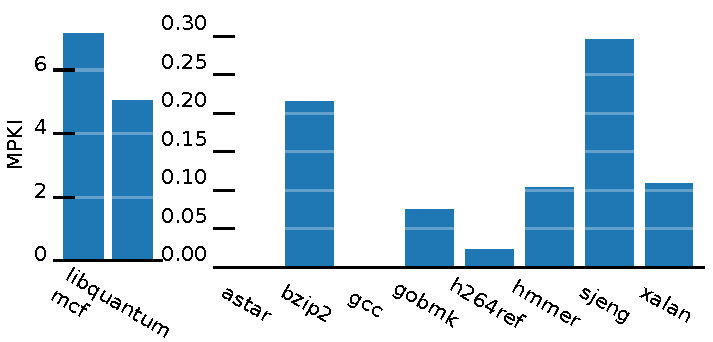
\includegraphics[width=3.4in]{figs/mpki_merged.pdf}
        \caption{Memory intensity of SPEC2006 benchmarks.}
        \label{fig:memstudy}
    \end{center}
\end{figure}

Figure~\ref{fig:performance} shows the performance overhead of full system 
protection as well as the overhead incurred by the changes to the memory 
controller (mc), the cache (waypart), the L3 to memory bus (membus), and the L2 
to L3 bus (L2L3) individually compared to the insecure baseline. The
overheads for libquantum and mcf, which are particularly memory intensive, are 
highest at 69\% and 18\% respectively. However, the arithmetic mean of the 
total overhead is quite low at roughly 9\%. Memory controller protection incurs 
by far the most overhead suggesting the impact on memory bandwidth is more 
significant than bus or cache underutilization. Overall, the results show that 
the timing compartments are viable for applications that require high assurance 
for software isolation.

\begin{figure}
    \begin{center}
        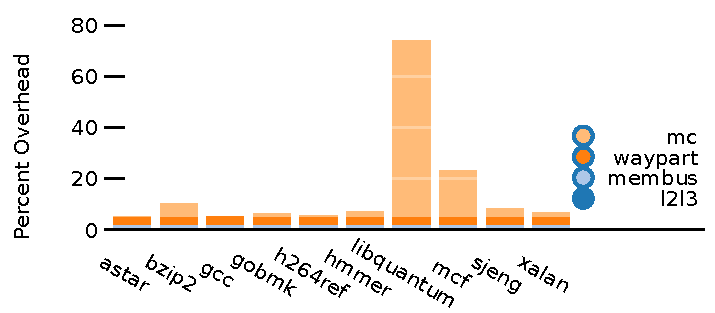
\includegraphics[width=3.4in]{figs/breakdown.pdf}
        \caption{Performance overhead for 2 TCs.}
        \label{fig:performance}
    \end{center}
\end{figure}

The performance overhead is likely to increase as the number of timing 
compartment scales up. To study the impact of the number of timing 
compartments, we evaluated the performance overhead with three and four timing 
compartments on a 4-core  processor, each occupying one core and private L1 and 
L2 caches. They share a 4MB L3 cache. We do not evaluate all permutations of 4 
benchmarks. Instead, we only evaluate the subset of these permutations where 
TC1, TC2, and TC3 are executing the same benchmark. As before, each of these 
workloads with the same program in TC0 is averaged.

The performance overhead as the number of timing compartments increases is 
shown in Figure~\ref{fig:scalability}. The arithmetic mean of the overheads for 
each benchmark for 2, 3 and 4 timing compartments are 9\%, 17\%, and 24\% 
respectively. For libquantum which is particularly memory intensive, the 
overheads are 76\%, 140\%, and 184\% for 2, 3, and 4 timing compartments. The 
results suggest that the overhead of timing timing channel protection is rather 
insensitive to the number of timing compartments for compute-bound 
applications. For memory-intensive applications, the overhead can increase 
noticeably. However, the results still suggest that timing compartments can 
allow distrusting software entities to share hardware and provide better 
overall performance than running them on separate dedicated machines.

\begin{figure}
    \begin{center}
        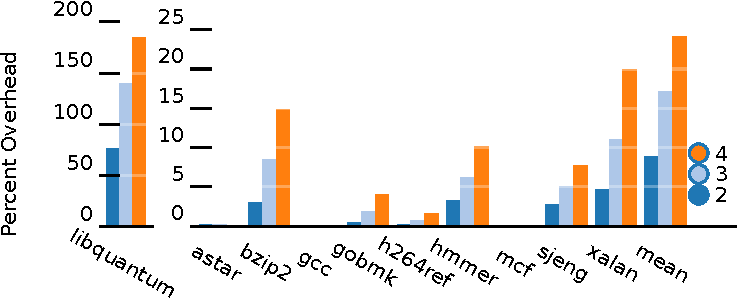
\includegraphics[width=3.4in]{figs/scalability_split.pdf}
        \caption{Performance overhead for 4 TCs.}
        \label{fig:scalability}
    \end{center}
\end{figure}

While future multi-core systems are likely to have a large number of processing 
cores, we note that many security applications will not require many timing 
compartments to be used concurrently. For example, the BYOD application only 
requires two TCs no matter how many cores exist in the system. Similarly, in 
a high-assurance cloud computing environment, the cloud provider can limit the
number of high-assurance virtual machines that can be located on each physical
system while increasing the system utilization by co-locating non-secure
virtual machines with high-assurance ones.


\section{Related Work}

Previous studies identified 
a number of microarchitectural timing channels 
caches~\cite{percival,bernstein,caseofaes,remoteaes,analyticalcache,collision,
deconstructing,cachegames}, branch predictors 
\cite{branchpred,predictingbranch}, processor
pipelines \cite{pipelines}, networks on chip~\cite{yaonocs,surfnoc}, and memory
controllers~\cite{ushpca14,fletcher-hpca14}. 
Also, people have proposed solutions for timing channels in
individual components such as caches~\cite{newcache,deconstructing}, memory
controllers~\cite{ushpca14,fletcher-hpca14}, and on-chip network
~\cite{yaonocs,surfnoc}.
However, the previous work has
so far focused on individual component. This work represents the first attempt
at designing a full microprocessor with complete internal timing channel protection.
Our integration efforts also exposed new sources of timing channels in module
interfaces such as MSHRs and cache/memory response ports.

%However, this paper presents the first microarchitecture to address all 
%internal microarchitectural timing channels. 

Ascend~\cite{ascend} proposes a
microarchitecture that aims to eliminate external timing channels so that
even untrusted software can execute without leaking any confidential
data. This presents a powerful option if physical attacks need to be
considered. However, Ascend does not allow a processor to be shared by
multiple software components at the same time, and does not address 
any internal timing channels.
Execution leases~\cite{execution_leases} 
provide another external timing channel solution at the hardware level by 
enforcing strict upper bounds on the execution times of program subsections. 

Timing channels are a form of information flow, and many approaches to 
controlling timing channels are based in information flow theory. Language 
level approaches track information flow and to either 
eliminate~\cite{quantleaks} or 
reduce~\cite{mitigation1,mitigation2,mitigation3} timing channels. At the 
systems level, information flow has been used to provide security 
through explicit channels ~\cite{flume-sosp07,histar-sosp06,laminar-pldi09}. 
These can be combined with timing compartments to provide total software 
isolation.

Work has also been done to verify hardware timing channel protection. GLIFT 
\cite{glift-asplos09} tracks all information flows, (including timing channels) 
in hardware at the gate level, though it does so at a high cost. GLIFT has 
later been used to develop information flow property checkers in gate level 
simulators ~\cite{glift-dac10,glift-dac11,glift-isca11}, and more recently 
hardware description languages that verify timing channel securtity 
~\cite{caisson-plas10,caisson-pldi11,sapper-plas13}.

\section{Conclusion}
This paper presents timing compartments, which provide an architecture 
abstraction to eliminate timing channels. When used in conjunction with access 
controls, timing compartments can provide total software-level isolation since 
other side or covert channel attacks require physical access. To realize 
timing compartments, we designed a full multiprocessor microarchitecture 
that eliminates all inter-program timing channels and evaluated it in the gem5 
architectural simulator. Our results show that the overheads are low.


% \title{
\vspace{-0.1in}
    Timing Compartments: An Architecture Primitive for Complete Software 
    Isolation
}

\ifanonymized{
    \author{}
}{
    \author{
    Andrew Ferraiuolo, Yao Wang, and G. Edward Suh\thanks{The first two authors 
    contributed equally to this work.}\\
    Cornell University\\
    Ithaca, NY 14850, USA\\
    \{yw438,af433,gs272\}@cornell.edu
    }
}


\date{}
\maketitle

\thispagestyle{empty}

\begin{abstract}

    %TODO

\end{abstract}

% \section{Introduction}

Timing channel attacks are becoming a major threat as hardware is increasingly 
consolidated and shared by distrusting entities, which traditionally have been
isolated on their own physical machines. For example, in cloud computing, mutually distrusting 
parties own virtual machines on shared hardware. In mobile devices, users often
run downloaded applications that cannot be trusted often handle private personal
information.
While untrusted applications can be sandboxed using
traditional access control mechanisms to limit explicit communications,
timing 
channels can still be used by a malicious program to extract or leak secrets.
%from other co-located applications.
Further, unlike physical side-channel attacks such as power analysis that require
physical proximity, timing channels can be exploited in software by remote
adversaries.

%For example, end users download untrusted 
%applications from the Internet which can then execute on the same hardware as 
%software that will handle the user's sensitive financial data. System on chip 
%platforms tightly integrate hardware designed by directly competing companies.  
%This necessitates hardware sharing among the drivers and proprietary algorithms 
%owned by these distrusting companies. 
%So timing channels 
%vulnerabilities are not only prevalent, but easy to exploit.

%Many of the systems that are vulnerable to timing channels do take security 
%measures to prevent explicit channel attacks. In a cloud platform, the 
%hypervisor performs physical address translation on behalf of the virtual 
%machines to isolate the virtual machines in the physical memory. Hypervisors 
%also use access controls to isolate virtual machines, typically relying on 
%hardware abstractions such as protection rings. However, these security 
%mechanisms are not enough. They do nothing to prevent coresident VMs from 
%leaking secret information through timing channels induced by hardware sharing.

In this paper, we investigate an architecture abstraction, named timing compartments (TCs),
which allows software to explicitly request strong timing isolation among software
entities that share a multi-core processor.
The goal of timing compartments is to remove fine-grained microarchitecture-level timing interference
that cannot be controlled in software and enable strong timing isolation that is
comparable to running a software entity on its own processor.
The timing compartment is designed to prevent both unintentional information leaks
through side channels and intentional leaks through covert channels.
%Using the timing compartments, software designers can specify a timing protection
%requirement that is necessary for each application. 
%More importantly, 
When coupled with software-level protection mechanisms to control timing channels 
through coarse-grained events such as scheduling and I/O, timing compartments
can enable comprehensive timing isolation of program or a virtual machine.

The timing compartment is designed so that timing isolation can be
separated from traditional access control. For example, multiple programs or
virtual machines that are isolated from each other using virtual memory may
be grouped into a single timing compartment if they either belong to the 
same trust domain or do not require timing channel protection. 
This separation provides a system the flexibility to only pay overhead for
timing channel protection when it is truly necessary.

To realize the timing compartments, a multi-core processor needs to be
re-designed to control inter-core timing interference in shared hardware
resources that cannot be efficiently controlled in software.
In this paper, we identify all resources that can be shared concurrently among
multiple cores on a typical multi-core processor, namely shared caches,
on-chip interconnect, cache coherence mechanisms, and off-chip memory controllers,
and augment each shared resource with a mechanism
to eliminate timing interference.

This ``full-processor'' protection study revealed new sources timing
channels on a multi-core processor that have not been studied yet.
For example, we found that interfaces between hardware modules and 
a cache coherence mechanism can lead to timing channels, and demonstrate
a covert channel attack using the coherence traffic interference.
The integration effort also showed that protection mechanisms need to
be carefully coordinated in order to avoid unnecessary inefficiencies.
To the best of our knowledge, this paper represents the first study
that implements comprehensive timing channel protection for a full 
multi-core microprocessor and evaluates the overhead.

%Recent studies have investigated mechanisms to prevent
%timing channels in various microarchitecture components, including
%shared caches \cite{icache,newcache,deconstructing,cachegames}, processor pipelines 
%\cite{pipelines}, branch predictors~\cite{branchpred,predictingbranch}, on chip 
%networks~\cite{yaonocs}, and memory controllers~\cite{ushpca14}.
%However, we found that the full timing channel protection for a multi-core
%processor requires more than simply integrating previous protection 
%mechanisms. Our study identified new sources of timing channels at
%interfaces between hardware modules and also found that protection
%mechanisms need to be coordinated together to avoid unnecessary inefficiencies.

%Ascend~\cite{ascend} considers external timing 
%channel attacks, but does not prevent timing channels due to shared resources.  
%Execution leases~\cite{execution_leases} provide an architecture abstraction
%that prevents external timing channels by bounding the execution time of a code 
%segment, but Execution leases do not prevent the internal timing channels 
%caused by shared hardware. GLIFT \cite{citation_needed} can be used to identify 
%timing channels, but does not prevent them. Further, the area, power, and 
%performance overheads are prohibitively large.

%Unlike previous work, timing compartments eliminate all internal timing 
%channels in a conventional microarchitecture. When combined with standard 
%access controls, timing compartments achieve the security of running mutually 
%distrusting software on separate hardware with some of the performance benefits 
%of sharing hardware. To the best of our knowledge, this is the first 
%architecture technique to reach this goal. This work is also the first to 
%experimentally evaluate the cost of applying timing channel protection to every 
%vulnerable component. Further, we show that integrating these protection 
%mechanisms to form a complete system with minimal performance overheads is 
%nontrivial and requires careful coordination. In the process of designing an 
%integrated timing channel protection system we identified two novel 
%microarchitectural timing channels. In addition to these contributions we 
%extend the taxonomy of timing channels and show how this taxonomy can be used 
%to identify techniques that can eliminate timing channels in any additional 
%components (e.g. accelerators).

The simulation results suggest that the performance overhead of supporting
timing compartments is relatively low, especially when the number of timing
compartments that simultaneously run is small.
%for the SPEC benchmarks. 
Even though
the timing compartments require shared resources to be statically 
allocated, the overall impact on the performance is limited by the fact
that the protection only affects infrequent cache misses and that modern
processors include large caches. 

The following summarizes the main contributions of the paper.

\begin{itemize}
\item The paper introduces a new abstraction that enables software to
explicitly remove microarchitecture-level timing interference on a multi-core.
The timing compartment enables new
applications that require strong timing isolation of software modules.
\item The paper identifies new timing channels on a multi-core processor,
including the one through cache coherence, and presents
comprehensive protection mechanisms for a full multi-core processor.
\item The paper shows how protection mechanisms need to be coordinated to
reduce the overhead of timing compartments.
\item The paper evaluates the performance overhead of the full-processor
timing channel protection, and shows that the overhead can be reasonable.
\end{itemize}

The rest of the paper is organized as follows.
Section 2 introduces timing compartments and 
presents example applications that can be enabled by strong timing isolation.
Section 3 identifies the sources of timing channels in a multi-core processor, and
describes protection mechanisms to eliminate them. 
Section 4 presents how the hardware protection mechanisms based on time-division
multiplexing need to be coordinated to reduce overhead.
Section 5 evaluates the proposed architecture. Section 6 discusses related
work, and Section 7 concludes the paper.

% \section{ Threat Model }

    The goal of this work is to completely isolate software modules that share
    hardware with one another. Virtual memory, processes, and machine 
    virtualization provide isolation through explicit channels. However, these 
    approaches to isolate software do not address timing channels that leverage 
    shared hardware. Interference in microarchitectural components can still 
    leak sensitive information.
    
    This is problematic for hardware/software architectures that rely on 
    software isolation to permit distrusting parties to share hardware. One 
    such example is platform as a service cloud computing wherein a hypervisor 
    controls virtual machines (VMs)
    which are leased to end-users. In this model, it is possible for a 
    malicious user to circumvent the isolation provided by virtualization and 
    extract secrets from a co-resident VM  through timing channels.

    Our approach to controlling timing channels is to group software modules 
    (such as VMs) into a hardware/software architecture primitive called a 
    timing compartment. A small, software trusted computing
    base sets up these timing compartments and initializes the hardware to 
    track actions performed on behalf of these timing compartments at the 
    hardware level. Then, the hardware architecture controls how the timing 
    compartments use shared resources to eliminate interference and provide 
    strong timing channel isolation. Timing compartments are described in 
    further detail in the following section. Intuitively, a single timing 
    compartment contains only software modules that trust each other (such as 
    all the VMs on a machine owned by the same user), however, timing channel 
    leakage between modules in different timing compartments must be 
    controlled.

    \begin{figure}
        \begin{center}
            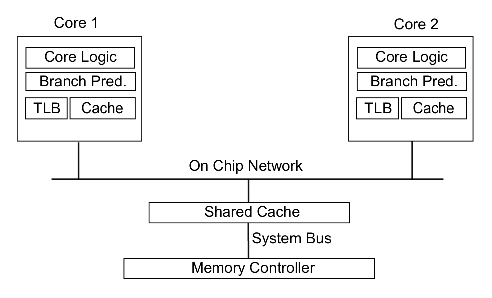
\includegraphics[width=3in]{figs/baseline.eps}
            \caption{The timing-channel vulnerable baseline architecture.}
            \label{fig:baseline}
        \end{center}
    \end{figure}

    Figure \ref{fig:baseline} shows a general hardware/software architecture on 
    which we base our threat model. The hardware architecture has multiple 
    cores, each with private resources such as a branch predictor, one or more 
    private caches, a TLB, and the core logic. Each processor is connected to a 
    shared cache through an on-chip network. The multicore processor is 
    connected to the main memory and a DMA module through the system bus. 

    The hardware is concurrently shared by multiple timing compartments. As 
    shown in Figure \ref{fig:baseline}, it is possible for a timing compartment 
    to have multiple software modules which may be allocated to different 
    cores. It is also possible for timing compartments to be time multiplexed 
    on the same core (e.g.  by context switching VMs), but it is not possible 
    for timing compartments to execute concurrently on the same core (e.g.  
    through SMT).
    
    The software monitor in Figure \ref{fig:baseline} is responsible for 
    setting up and managing the timing compartments and initializing the 
    hardware mechanisms that control them. This software monitor must be 
    trusted as each timing compartment must rely on it. Similarly, the hardware 
    itself is trusted and attacks that require physical possession of the 
    hardware are not addressed by this work.

% \section{Timing Compartments}

This section introduces a new architecture abstraction, named timing compartment.
We first discuss the type of timing channels that the timing compartment is designed
to prevent. Then, we define the timing compartment, describe our threat model,
and discuss application scenarios that the timing compartments can enable.


\subsection{Taxonomy of Timing Channels}

%    \begin{figure}
%        \begin{center}
%            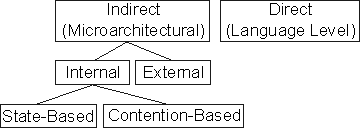
\includegraphics[width=2.2in]{figs/taxonomy.pdf}
%            \caption{The taxonomy of timing channels}
%            \label{fig:taxonomy}
%        \end{center}
%    \end{figure}

A timing channel represents a security vulnerability where the timing of events
depend on confidential information. An adversary can use timing channels as
side channels to learn secrets such as cryptographic keys or passwords or as
covert channels to intentionally bypass restrictions on communications.

%Figure~\ref{fig:taxonomy} summarizes the taxonomy of timing channels. \emph{Direct} or 
%language level timing channels can be identified by examining the source code 
%\cite{mitigation3}. A password checking algorithm that stops as soon as an 
%incorrect character is found causes a direct timing channel that leaks 
%information about the correct password. In contrast, \emph{indirect} or 
%microarchitectural timing channels cannot be identified in the source code 
%since they depend on hardware level behavior \cite{mitigation3}. Conventional 
%caches cause an indirect timing channel whenever the probability of a cache hit 
%depends on secret data. Programming language techniques have been developed to 
%address language level timing channels 
%\cite{timesens,mitigation1,mitigation2,mitigation3}. It is possible to reduce 
%the information leaked by some microarchitectural timing channels at the 
%language level \cite{mitigation3}. However, eliminating all leakage caused by 
%microarchitectural timing channels is difficult without hardware support.
%%%% More precise, wordier version:
%  However, efficiently providing strict timing-sensitive noninterference in 
%  the presence microarchitectural timing channels without the support of 
%  hardware is a hard problem.

Timing channels can be categorized into {\em external} and {\em internal} 
\cite{mitigation3}. 
External timing channels exist when the timing of a program's event that
can be observed externally leak information on data that the program processes. 
For example, a password checking program that sequentially compares strings
and stops on the first incorrect character leaks where a mismatch is.
As another example, Bernstein's attack~\cite{bernstein} exploits data-dependent
timing variations in a popular implementation of an AES encryption.
%Adversaries can carry out external timing channel attacks even without sharing 
%hardware with a victim program. 
Because the external timing channels happen when a program's operation differs
depending on a secret, language-level techniques have been developed to
mitigate them \cite{timesens,mitigation1,mitigation2,mitigation3}. 

%further divided into internal or 
%external timing channels. \emph{External} timing channels are not caused by 
%interference, and are exploited by an adversary that directly measures the 
%timing of the victim's actions. External timing channels can be exploited by an 
%adversary that does not share hardware with the victim. Bernstein's 
%attack~\cite{bernstein} exploits an external timing channel in popular 
%implementations of AES (such as OpenSSL). The external timing channel exists 
%because the cache access pattern both affects the overall execution time of the 
%AES implementation and depends on the secret key. The adversary carries out the 
%attack without sharing any hardware by directly measuring the response times of 
%the victim machine.
%%%%% The long explanation
% The adversary uses a copy of the same AES implementation as the victim to 
% time the encryption of a number inputs with a known key on the adversary's 
% local machine. Then, the adversary makes requests to the victim machine using 
% the same inputs and times how long the victim machine takes to encrypt the 
% inputs with an unknown key. In both cases, the execution time depends on the 
% cache access pattern which depends on the key. The adversary can use the 
% timing information gathered with the known and unknown keys to learn the 
% secret AES key.

Internal timing channels exist when one program's timing depends on another
program that shares the same hardware due to interference. In this case,
an adversary can exploit the timing channel by measuring the timing of its
own events even without directly observing a victim program.
For example, Percival~\cite{percival} showed an internal timing channel
through a shared cache where an attack program can extract an AES key
by measuring its own cache access time, which reflects a victim program's
cache accesses that depend on the key.



\subsection{Definition of Timing Compartments}

A timing compartment is a new architecture abstraction that allows software to
explicitly control {\em internal timing channels} that exist in shared systems. 
The ability to control timing channels, combined with a traditional access
control mechanism such as virtual memory, enables complete software isolation
because the timing channel is the only form of side/covert channels that can be
exploited in software without physical attacks.

From the software perspective, a timing compartment consists of one or more software 
entities such as threads, processes, and virtual machines. 
Then, software can express a policy that specifies which timing channels among
timing compartments are allowed or not. In general, the policy can take a form
of a lattice model, which defines ordering between security levels \cite{denning}.
This lattice model is quite expressive and widely used for information flow control. 
For example, the lattice may restrict timing channels only in one direction 
from $\mathtt{TC1}$ to $\mathtt{TC2}$ ($\mathtt{TC2} \leq \mathtt{TC1}$).
The lattice may disallow any timing channel between two compartments by making
them incomparable ($\mathtt{TC_1} \nleq \mathtt{TC_2}$, $\mathtt{TC_2} \nleq \mathtt{TC_1}$).

%Here, a software 
%entitiy is some system abstraction (such as processes or threads in a single OS 
%system or virtual machines in a virtualization based system) that execute 
%software and have an owner. Intuitively, a single timing compartment contains 
%only software entities that trust each other explicitly (such as all the VMs on 
%a machine owned by the same user) or implicitly (all the VMs that do not want 
%to pay for protection), and leakage within a timing compartment is safe.

Similar to other architecture abstractions such as virtual memory, the
timing compartments need to be implemented as a combination of hardware-software
mechanisms. The underlying hardware must provide mechanisms to distinguish
events from different timing compartments and control timing interference 
in shared resources.
Then, a trusted software component needs to manage the hardware mechanisms 
at run-time. We call this trusted software as timing compartment manager (TCM).

%To enforce the policy, a trusted software component called the timing 
%compartment manager (TCM) confines software entities into TCs. The TCM then 
%informs the hardware of the TCs and policy. At runtime, the TCM tags software 
%requests for hardware to indicate the TC of the software entity that made the 
%request. The hardware then enforces the policy by controlling how requests from 
%different TCs share resources.

The timing compartments allows software to explicitly control timing channels
among groups of software entities, but does not enforce any restrictions within
each compartment. We believe that handling timing channels separately from
traditional isolation abstractions such as processes and virtual machines is essential
to allow efficient system designs. Because timing channel protection is more expensive
than traditional access control, a designer should be able to pay the overhead
of timing control only when truly necessary.

%Timing compartments only address timing channels; they do not control 
%information flow through explicit channels. Handling these concerns separately 
%allows for more flexibility in the overall system design.  When designing a 
%secure system, implementors must consider how the cost required to carry out a 
%particular attack compares with other attacks, the potential damage that could 
%be caused by an attack, and the cost and performance impact of implementing the 
%security mechanisms needed to stop it. This enables timing compartments to 
%provide timing channel protection only to software entities that need it.

\subsection{Threat Model}

%Goal
The goal of the timing compartment is to enable complete software isolation
on shared hardware, comparable to having separate hardware for each.
%Assumptions
In that sense, we assume that a target system has multiple cores with shared
resources such as caches, on-chip interconnect, and off-chip memory that can
be used by multiple programs concurrently. The system can also be time multiplexed.
%The multicore system of interest consists of hardware resources that are
%concurrently shared by multiple software entities. It is possible for software 
%entities to be time multiplexed on the same core (e.g.  by context switching 
%VMs), but the system does not allow software entities to execute concurrently 
%on the same core (e.g. through simultaneous multithreading). 
We also assume that there exists a trusted software layer such as an OS or a hypervisor,
which provides conventional software isolation for explicit communication channels.
The timing compartment manager (TCM) is assumed to be a part of this trusted software.

%Attacks we handle.
%However, these approaches to isolate software do not address timing channels 
%that leverage shared hardware. To guarantee total isolation, internal timing 
%channels must also be eliminated. We eliminate all internal microarchitectural 
%timing channels including state and state-based timing channels. 
%This includes 
%all timing channels caused by concurrently shared resources as well as timing 
%channels in hardware that is shared through time multiplexing (e.g. by context 
%switching).

The timing compartment aims to eliminate {\em internal} timing channels through
interference in shared microarchitecture resources. In particular, the goal is
to prevent both unintentional (side channels) and intentional (covert channels)
information leaks.
However, external timing
channels, which exist even with dedicated hardware, are not prevented by the
timing compartments. If necessary, the external timing channels can be controlled 
in software. 
Similarly, timing channels through I/O devices are not considered in this study
because their accesses can be controlled in software.
Finally, we not consider physical attacks on the system such as
physical side-channel attacks through power consumption or electromagnetic emission. 

%Attacks we don't handle.
%Since our goal is to address vulnerabilities 
%caused by hardware sharing,
%timing channels that are external to the hardware are not addressed.
%Any timing channels that are external to the hardware in this system would also 
%be present if the software entities executed on separate hardware. If 
%necessary, external timing channels can be controlled in software. Similarly, 
%we do not address language level timing channels since these may also be 
%addressed in software.  Lastly, we do not consider physical attacks and assume 
%that the adversary does not have physical access.


\subsection{Application Scenarios}

The ability to control internal timing channels can significantly increase a level of
assurance in a number of applications where distrusting entities share a
physical system. Here, we briefly discuss representative applications.

\subsubsection{Bring Your Own Device (BYOD)}

As mobile devices such as smartphones and tablets are becoming widely used, 
companies and government organizations are starting to allow employees to
use their own devices to access corporate data. This trend is often called
Bring Your Own Device (BYOD). However, there is a major concern that such a
mixed use can lead to a leak of confidential data through personal emails or
downloaded applications. Today's BYOD solutions such as Samsung Knox uses
software containers or virtualization to separate the two environments:
personal and work. Yet, these solutions cannot prevent information leaks
through internal timing channels.

\begin{figure}
    \begin{center}
        \includegraphics[width=1.51in]{figs/app_byod.pdf}
        \caption{A BYOD example.}
        \label{fig:app_byod}
    \end{center}
\end{figure}

The timing compartment enables a strong isolation guarantee in the BYOD
scenario. For example, consider the solution based on virtualization as 
shown in Figure~\ref{app:byod}. In this case, the virtual machines for
work and personal use can be assigned to two different timing compartment:
$TC_{work}$ and $TC_{pers}$. Then, the lattice can be set so that no
information can flow from $TC_{work}$ to $TC_{pers}$.
Note that the BYOD application only requires two timing compartments even
though a system may have many cores and run many applications.

\subsubsection{High-Assurance Cloud Computing}

In cloud computing such as Amazon EC2, virtual machines (VMs) from multiple
distrusting clients often share physical machines. 
%A cloud provider 
%co-locates many VMs on a single machine to increase its utilization,
%and tenants often have little control over where their VMs run. 
For example, a tenant may share hardware with competitors or attackers that 
want to extract sensitive data. Today's virtualization technologies restrict 
explicit communication channels among virtual machines, but cannot control 
internal timing channels. In fact, recent studies have shown that timing channels
can be exploited in commercial clouds to extract secrets such as 
a password \cite{FIXME}.
For some clients, timing channels may not be a major concern. Yet, for enterprise
or government clients who require high assurance, this security threat makes
public cloud computing not an option. 

\begin{figure}
    \begin{center}
        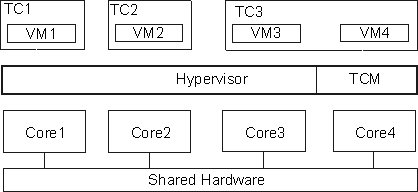
\includegraphics[width=2.79in]{figs/cloud_tcs.pdf}
        \caption{A cloud computing example. VM1 
        and VM2 have high security requirements, but VM3 and VM4 do not.}
        \label{fig:cloud_tcs}
    \end{center}
\end{figure}

The timing compartment can enable high assurance cloud computing by ensuring that
there cannot be unintended information leak among virtual machines.
Figure~\ref{fig:cloud_tcs} shows an example with four virtual machines (VMs).
%that have different security requirements. 
VM1 and VM2 require a strong isolation guarantee and distrust other VMs.
VM3 and VM4 run low-security applications that are not concerned with timing channels
but require high performance. The figure shows that three timing compartments can
be used to meet the security requirements in this example.
VM1 and VM2 are placed in their own timing compartments $TC1$ and $TC2$, but 
VM3 and VM4 are grouped in $TC3$. The lattice can be set so that VM1 and VM2
cannot leak information to any VM but no constraint is put on VM3 and VM4:
$TC3 \leq TC1, TC3 \leq TC2, TC1 \nleq T2, TC2 \nleq TC1$.
%TC3 preceeds both TC1 and TC2 implying timing channel leakage from VM3 or VM4 to 
%any other VM is not controlled. However, VM1 and VM2 cannot leak information to 
%VM3 or VM4. Additionally, VM1 and VM2 cannot leak information to each other 
%since TC1 and TC2 are incomparable. This meets the security requirements of VM1 
%and VM2 since both are totally isolated from the other VMs through timing 
%channels. Since VM3 and VM4 share a timing compartment, they can share 
%resources normally and incur minimal performance overheads.


\subsubsection{Untrusted Software} 

The ability to completely eliminate timing channels enables timing compartments
to be used to contain information even when software is potentially malicious.
For example, today's smartphone users often rely on many third party applications
that cannot be fully trusted to manage private or sensitive data. A system may
sandbox an untrusted application and restrict its communication channels
when it accesses sensitive data. However, today's access control mechanisms cannot
prevent the untrusted application from leaking information to another unrestricted
application through internal timing channels. The timing compartment can be added 
to provide a complete sandbox. 
In the cloud computing context, the same timing channel protection can be used
by a cloud provider to sandbox a third-party web services that cannot be fully trusted.

\subsubsection{Safety-Critical Systems}

In addition to protecting confidential data, the capability to control interference
in shared hardware can also be used to provide timing guarantees on safety-critical systems.
For example, hard real-time systems such as automotive controllers must meet
strict timing requirements. Unfortunately, today's multi-core processors provide
no timing guarantee when shared by multiple programs. The timing compartment can be
used to ensure that the timing of safety-critical components are not affected by
the rest of a system.


% \section{Microarchitectural Timing Channels and their Sources}
\label{sec:tc_sources}
The baseline architecture is vulnerable to microarchitectural timing channels 
caused by shared resources including the private and shared caches, the on chip 
network, the system bus, and the main memory. Furthermore, data-dependent 
variations in the timing parameters of microarchitectural components can cause 
timing channels even in the absence of sharing. In general, all 
microarchitectural timing channels may be classified as state based timing 
channels, resource contention based timing channels, or direct observation 
timing channels. As we will show, the classification of a timing channel within 
this taxonomy directly implies which techniques may be used to control that 
channel. We later present approaches to address timing channels of each kind.

In a state based timing channel:
\begin{itemize}
    \item The time required to access a resource with state depends on the 
        contents of that state (i.e. it depends on previous system behavior).
    \item An adversary can observe the time required to complete requests to 
        that resource made by one software module(that it controls).
    \item Another software module operating on secret data can modify this 
        state, and these modifications can possibly affect the request timings 
        observable by the adversary.
    \item These modifications can possibly depend on the secret.
\end{itemize}
When all of these conditions are met, the timings that the adversary can 
observe correlate with the secret, and sensitive information may be leaked.

There is a resource contention based timing channel whenever:
\begin{itemize}
    \item A resource can concurrently service a finite number of requests and 
        this limitation can affect the time required to service a request (e.g.  
        if a request can be delayed because the resource is servicing another 
        request) regardless of state or previous system behaviour.
    \item An adversary can observe the time required for requests to that 
        resource made by one software module (that it controls).
    \item Another software module that directly operates on a secret contends 
        for the same resource and this contention can affect the timings 
        observable by the adversary.
    \item Usage of this resource by the software module operating on the secret 
        can possibly correlate with the secret.
\end{itemize}
Together, these conditions imply that the adversary can make requests to use a 
resource with a contention based timing channel and extract secrets from these 
timings. If a timing channel can satisfy the definition of a state based timing 
channel, it should not be considered a resource contention based timing 
channel.

If instead the adversary can directly observe the time required for the 
software module operating on a secret to complete any action (e.g. run an 
entire program or complete a memory request) that may be correlated with some 
secret, this is a direct observation timing channel. If the adversary can 
exploit the timing channel by measuring the timing of its own actions, it is 
not a direct observation timing channel. Note that in state based and resource 
contention based timing channels an adversary can only measure the timings of a 
software module that it controls, but not the timings of the software modules 
directly operating on a secret. The sets of direct observation, resource 
contention, and state based timing channels are strictly disjoint.

Direct observation timing channels are distinct from the seemingly similar 
external timing channels. An external timing channel is one that is exploited 
by an adversary that makes timing measurements from outside of the system (i.e.  
by an adversary that does not share any hardware with the victim) whereas an 
internal timing channel is exploited through measurements made within the 
system. In Bernstein's attack \cite{bernstein}, the adversary exploits the 
timing channel by sending requests to a remote system and measuring the time 
required to complete the request. This is an external timing channel since the 
victim resides on a separate machine from the adversary, and it is a direct 
observation timing channel since the adversary is measuring how long the victim 
machine takes to fulfill a request. However, not all direct observation timing 
channels are external. Suppose the system of interest is based on a TrustZone 
like system and a normal world application must make requests of the secure 
world to execute correctly. An adversarial normal world application can make 
requests of the secure world and measure the time required to fulfill the 
request. Since fulfilling the request is an action carried out by the victim 
rather than the adversary this is a direct observation timing channel, but 
since the adversary and victim share hardware the timing channel is internal.

The rest of this section classifies the timing channel vulnerabilities due to 
each microarchitectural component into this taxonomy, and provides elucidating 
examples of these classes of timing channels. Note that a microarchitectural 
component may cause multiple timing channels which may be of a different class 
necessitating countermeasures to address each channel.

\subsection{Private Caches}
\label{sec:priv_cache}
The baseline private caches are shared among software modules whenever a core 
context switches between them. Despite the lack of concurrent sharing, private 
caches cause information leakage between context switches and through variation 
in timing not due to sharing.

Private caches impose a state based timing channel even if each software module 
has a totally disjoint address space (i.e. no software module can read or write 
any memory address that another software module can read or write). Requests to 
the memory hierarchy for addresses that are stored in the cache (cache hits) 
are returned faster than requests that are not stored in the cache (cache 
misses). So, the time required to access the cache depends on its state. An 
adversary controlling a software module can use conventional time measurement 
libraries to record cache access timings and determine which requests are hits.
The adversary controlled software module can be context switched out for one 
that will operate on some secret. This other can read new memory addresses into 
the cache which may evict some of the old entries that occupied the cache. The 
memory addresses used by this module can depend on the actual data of the 
secret, for example, through a branch condition. (In the attack proposed by 
Bernstein \cite{bernstein} the addresses read by an AES algorithm depend on the 
secret key through sboxes). Therefore, this satisfies the definition of a state 
based timing channel.

The adversary can exploit this timing channel by loading an array from memory 
that occupies as many cache lines as possible. The adversary then waits until 
the virtual machine he or she controls is context switched out and replaced 
with the software module that will operate on the secret. This software module 
may evict some of the cache lines of the array. When the adversarial software 
module context switches back, the adversary can learn which cache lines were 
evicted by making requests to read each element of the array and measuring the 
timing. It will take longer to read the elements which were evicted. Unless the 
cache is fully associative, the particular cache lines that were evicted will 
depend on the addresses operated on by the victim software module. Even if the 
cache is fully associative, the adversary can use an array that completely 
fills the cache and learn the number of cache lines read by the adversary - a 
quantity that can also depend on a secret.

Additionally, private caches also cause direct observation timing channel 
vulnerabilities if the adversary can measure the duration of an event performed 
by a software module that operates on some secret and includes one or more 
private cache
accesses. In the DRM video playback usage case, an example of such an event is 
a function call in the secure world that handles a request made by the normal 
world. The adversary can measure the time between making the request (invoking
the monitor to context switch the adversarial software module out) and being 
context switched back in. The total time required to complete the function will 
depend on the cache hit ratio which depends on program control flow and 
therefore possibly the secret. This direct observation timing channel has the 
interesting property in that it requires no interference or resource sharing 
between the two software modules at all.
 
\subsection{TLBs and Branch Predictors}
As with private caches, TLBs are shared among software modules between context 
switches. The TLB effectively caches address translations, and since page table 
hits are faster than misses, it can be shown through similar reasoning as 
Section \ref{sec:priv_cache} that the TLB causes state based timing channels 
and direct observation timing channels. The branch predictor is also shared by 
software modules between context switching. It stores branch prediction history 
in a branch prediction table, the contents of which are used to decide whether 
or not a branch should be taken. This prediction can positively or adversely 
affect execution time, and space in the branch prediction history table is 
finite, so evictions must be made. Again, similar reasoning can be applied to 
see that the branch predictor also causes state based and termination timing 
channels.

\subsection{Shared Caches}
Shared caches cause timing channel vulnerabilities that are similar to the 
vulnerabilities of the private caches (the state based timing channel and the 
direct observation timing channel). However, unlike the private caches, shared 
caches are subject to interference due to concurrently executing software 
modules. This allows the attacker to have finer-grained control over when 
interference takes place, potentially allowing for faster exfiltration of 
secrets. However, since the shared cache is larger it has a higher access time, 
and since it is higher in the memory hierarchy the private cache reduces the 
chance of a shared cache access. Both of these factors decrease the 
exfiltration rate, so it is unclear if shared cache timing channels are more 
efficient than private cache timing channels.

\subsection{CPU Logic}
There is a direct observation timing channel here as we discussed. This is just 
a placeholder for now.

\subsection{Main Memory}
The main memory is shared between concurrently executing software modules, and 
analogous to the timing disparity between cache hits and misses, page faults in 
main memory take substantially longer than accessing entries that are present 
in main memory. So the main memory has sources of timing channels that are 
similar to the shared cache. However, the memory controller has additional 
timing channels due to resource contention as well as other state based timing 
channels. Wang et. al. classify timing channel sources as queueing structure 
interference, scheduler arbitration interference, and DRAM device interference.  
In this section these timing channel sources are summarized, and it is shown 
that the timing channels of the memory controller may also be thought of as 
resource contention or state based timing channels.

The DRAM device contains several finite resources (e.g., the command bus, data
bus, banks, and ranks), and contention for these resources is resolved by the 
queueing structure and scheduler. Each of these resources causes a resource 
contention based timing channel that may be observed in both the queing 
structure and scheduler. For example, two requests to the same bank cannot
be scheduled at the same time causing a timing channel observable in the 
queueing structure. Suppose the queueing structure contains a request from a 
victim owned software module for a bank. If an adversarial software module 
issues a request to the same bank, it will be delayed, informing the adversary 
that such a victim request exists.  Similarly, contention for the command bus 
causes a timing channel that may be observed in the scheduler. If a request 
from one software module arrives at the scheduler in the same cycle as a 
request from another software module and for a different bank, one of the 
requests is scheduled and the other is delayed since only a single command can 
occupy the command bus at a time.

A memory controller queueing structure collects incoming requests for the DRAM 
and stores them in a queue until. As noted, timing channels due to contention 
for resources in the
DRAM may be observed in the queue. However, even if these timing channels are 
closed, there is still a distinct state based timing channel in the queue. To 
see this, suppose the resources of the DRAM are no longer finite, that is, the 
ranks, banks, command bus, and data bus can each handle infinitely many 
requests at the same time. (Though one may argue that the queue is no longer 
necessary at all under these circumstances, practical techniques to address the 
aforementioned channels do not involve infite resources and queues will still 
be necessary. The intent here is merely to show that there is still a distinct 
timing channel even in the absennce of this resource contention).
The state elements of the queue can accommodate only a finite number of 
requests. If the queue is completely filled, any incoming request must be 
stalled. Therefore, the time required to make a memory request depends on the 
state in the queueing structure. An adversary can measure the time required for 
its memory requests and learn if a victim software module has completely 
occupied the queue or not (since the delay will be greater if the queue is 
full). This can indicate whether or not a secret dependent control flow segment 
led the victim program to a memory intensive region of of the program or not.  
These conditions imply that the finite queue space induces a state based timing 
channel. Note that although one might be inclined to think of queue slots as 
finite resources, the timing varition that is observable here depends on the 
system behavior in previous cycles so it is not a resource contention based 
timing channel.

The resource contention timing channels for the ranks, banks, and buses may be 
observed in the scheduler as well. However, there is another distinct state 
based timing channel. Depending on the specific scheduler policy, one request 
will be issued by the scheduler potentially causing other requests to be 
delayed.  Often, this policy is designed to exploit row buffer locality. When a 
memory access takes place, the row being accessed is stored in a row buffer 
(sense amplifier). Accesses to rows that are already stored in the row buffer 
are faster than those which are not. The decisions made by the scheduler depend 
on this state (and therefore the behavior of the system in previous cycles).  
This causes a state based timing channel.

\subsection{On Chip Network \& System Bus}
This section must still be completed, but it is likely that these timing 
channels can be viewed as resource contention based timing channels.

% \section{Timing Channel Protection Mechanisms}
This section proposes mechanisms that prevent all microarchitectural timing 
channels. At a high level, our approach to handling state-based timing channels 
is to apply static partitioning (or flushing where appropriate for resoureces 
that are private to a core), and our approach to handling resource contention 
based timing channels is to use time division multiplexing. Direct observation
channels are resolved by determining a worst case time for the victim 
observation and always returning at the worst case time. By classifying a 
timing channel with the proposed taxonomy, one can directly find a high level 
approach to address it. 

\subsection{State Based Timing Channel Protection}
\subsubsection{Static Partitioning}
The private and shared caches, TLBs, and branch predictors of each core in the 
system induce state based timing channels. These timing channels can be 
eliminated by allocating static partitions to each timing compartment in the 
state of each of these resources. In states where entries may be evicted (e.g.  
caches and TLBs), a timing compartment may only evict entries in its own 
partition (and it may not evict entries of another partition even if the other 
partition has a lower security level).

This technique applied to the cache eliminates attacks that attempt to observe 
cache line evictions. Formerly, an adversary that controls one timing 
compartment could load a large array into the cache and observe which entries 
are evicted by the other domain. Now, if an adversary attempts the same attack, 
it will only be able to fill cache lines in its own domain and the other domain 
can only evict cache lines in its own domain. So, the adversary learns nothing 
with this attack. The same reasoning applies to attacks based on branch 
predictor table capacity and TLB entry eviction. For each of these 
microarchitectural timing channels, the timing compartment operating on a 
secret cannot make any modifications to the state that are observable by any 
other domain. This implies the state based timing channel has been eliminated.

\subsubsection{Flushing}
The private caches, TLBs, and branch predictors have the unique property that 
they are only shared among timing compartments between context switches. We can 
leverage this by flushing the state elements in each of these whenever  a 
context switch happens rather than statically partitioning them. This increases 
the maximum space a timing compartment can consume at a given time, but when a 
context switch happens there are two performance penalties. The time required 
to perform the context switch potentially increases if flushing the state 
cannot be done instantly or in parallel with other steps, and there is a 
penalty in performance due to the actual loss of state. In the private cache, 
this performance loss is a sequence of compulsory cache misses - misses that 
cannot be avoided at the beginning of execution because the cache is empty - 
that lasts until the cache is refilled with data that is useful to the current 
timing compartment. The TLB similarly suffers from a now empty table of address 
translations, and the branch prediction accuracy is weakened by a loss of 
history. 

Clearly there is a tradeoff between these two approaches. If context switches 
are expected to be infrequent (as may be the case if the timing compartments 
are not working together and the context switches are due to normal hypervisor 
management), it is likely that flushing is preferable since the performance 
loss will also be infrequent. However, if the context switches happen often (as 
in the case of the DRM processor with only a single core that context switches 
out the normal world any time the secure world must handle a request) the 
performance impact of the lost state and flush time may be more significant 
than that of the capacity lost to partitioning.

\subsubsection{Flattening}
The last technique to addressing state based timing channels eliminates the 
dependence of access time on the state by making every access take the same 
amount of time. This can be applied to a cache by treating every access as a 
cache miss. This is equivalent to eliminating the cache entirely. This has dire 
performance implications and is not likely an effective solution to address 
cache induced state based timing channels. However, this flattening technique 
is a suitable solution for the state based timing channel in the row buffer of 
the memory controller. Static partitioning cannot sensibly be applied to the 
row buffer since it contains exactly one row. Unlike caches and other state 
based timing channels, the performance lost from neglecting the caching effect 
of the row buffer is tolerable. Flattening may be applied to the row buffer by 
using a closed page row buffer management policy.

\subsection{Resource Contention Based Timing Channel Protection}
\subsubsection{Time Division Multiplexing}
This section is not yet completed, but we already know how this applies to 
memory controllers and on chip networks, so this is just a matter of writing.

\subsection{Direct Observation Protection}
Direct Observation channels are problematic for certain usage scenarios (such 
as the DRM processor) where an adversary can observe the timing of an action 
taken by a victim timing compartment action directly.  The private and shared 
caches, TLBs, branch predictors, and memory controller all induce direct 
observation channels whenever the adversary can observe the time required to 
complete an action that depends on a secret and is comprised of one or more 
requests to use one of these resources.  In the DRM processor, the normal world 
makes requests for the secure world to perform some function. An adversarial 
normal world can measure the time it takes for this request to be handled, and 
handling the request may depend on any number of requests to use any of the 
aforementioned resources. In general, this timing channel can be addressed by 
finding a conservative upper bound on the action that causes the direct 
observation channel. The action must be forced to appear to take the worst case 
time on each execution. In the DRM processor case, this means a worst case time 
estimation for each secure world operation must be found before execution. 
Then, whenever a secure world operation would normally terminate before the 
worst case time, it must be stalled until the worst case is reached.

% \section{Implementation}
\subsection{Shared Cache}
\subsection{Memory Controller}
\subsection{On Chip Network \& System Bus}
\subsection{Handling Context Switches}

% \section{Evaluation}

We evaluated the timing compartments architecture using the gem5 architectural 
simulator~\cite{gem5} integrated with the DRAMSim2~\cite{DRAMSim2} 
memory simulator. Our experiments use multiprogram workloads 
comprised of SPEC2006 benchmarks compiled for the ARM ISA. 

Table~\ref{tab:config} shows our system configuration.
The cores use the gem5 ``O3`` out-of-order core model which runs at 2GHz. 
Each core has private 32KB L1 instruction and data caches, and private 256KB L2 
cache. The cores share a 4MB L3 cache. We derived cache configuration 
parameters from the Intel Xeon E3-1220L, which is a two core architecture used 
by Amazon EC2. In DRAMSim2, we simulate a 667MHz 2GB DDR3 memory. The 
interconnects in the simulator runs at 1GHz. Unless specified otherwise, each experiment is 
fastforwarded for 1 billion instructions, and run for 100 million 
instructions. We will first describe our security evaluation and then show
the performance evaluation.

\begin{table}
    \caption{Simulator configuration parameters.}
    \centering
    \begin{tabular}{|l|l|l|r|}
        \hline
        \multicolumn{3}{|l|}{gem5 core model} & ``O3''        \\\hline
        \multicolumn{3}{|l|}{CPU Clock}    & 2GHz             \\\hline
        \hline
        \multicolumn{2}{|l|}{Memory}             & 2GB    & 667MHz  \\\hline
        \hline
        \multicolumn{3}{|l|}{Network Clock}      & 1GHz \\\hline
        \hline
        L1d / L1i  & 32kB   & 2-way  & 2 cycles\\\hline
        L2         & 256kB  & 8-way  & 7 cycles \\\hline
        L3         & 4MB    & 16-way & 17 cycles  \\\hline
    \end{tabular}
    \label{tab:config}
\end{table}

\subsection{Security Evaluation}

To experimentally evaluate the security of the timing channel protection in our 
architecture, we use a two-core system with two timing compartments, TC0 and
TC1, running concurrently. The protection policy is configured to disallow any 
timing channels between the two compartments. If the number of cycles required 
to execute a certain number of instructions for a particular benchmark running on 
TC0 depends on which benchmark is running on TC1, it indicates timing 
interference exists that can be exploited to leak information about TC0. A 
secure system should guarantee the benchmark running in TC0 always uses the 
same number of cycles to finish regardless of which benchmark TC1 is running. 

Using the rule above, we evaluated the security of our architecture by running 
a fixed benchmark on TC0 while varying the benchmark on TC1. Then we compared 
the total execution time for the fixed benchmark in different runs. We 
evaluated our architecture as well as the baseline insecure architecture which 
does not implement any protection. As expected, the results for the baseline 
show the execution time of a particular benchmark on Core 0 changes significantly 
depending on the benchmark on Core 1, indicating timing channels exist between
the two cores. On the other hand, when running each pair of benchmarks with 
timing channel protection we observed no execution time difference by changing 
which program runs concurrently with TC0.

\subsection{Performance Evaluation}

The timing compartment architecture extends the insecure baseline with
static partitioning and time multiplexing to secure the shared hardware 
resources. These changes lead to underutilization, and thus, a performance
overhead. To evaluate the performance overhead, we ran pairs of
SPEC2006 benchmarks, and measured the execution time of the benchmark
in TC0. Since the timing channel protection mechanisms primarily affect the memory 
hierarchy, the memory intensity of the benchmarks is related to the performance 
overhead.
The memory intensity of each benchmark, in memory requests per thousand 
instructions, during the program segment used for our experiments is shown in
Figure~\ref{fig:memstudy}. Of the SPEC2006 benchmarks, mcf has the most memory 
requests, while astar has none after fast-forwarding for 1B instructions.

For the baseline architecture, we calculate the average execution time of the 
benchmark on Core 0 by averaging among runs with different benchmarks on Core 1. 
The execution time of the benchmark in Core 0 is impacted by the benchmark in 
Core 1. In the timing compartments architecture, the execution time of TC0 (on 
Core 0) is independent of workloads running in other timing compartments.

\begin{figure}
    \begin{center}
        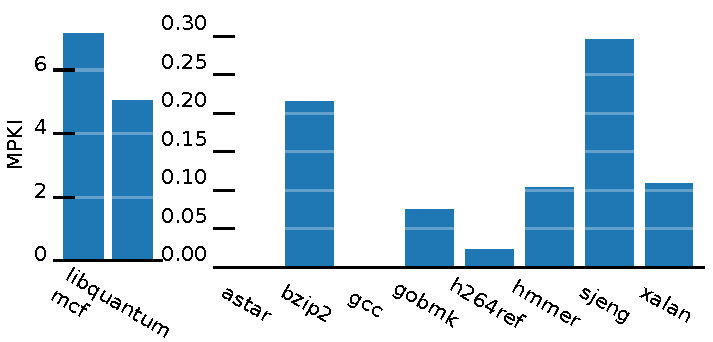
\includegraphics[width=3.4in]{figs/mpki_merged.pdf}
        \caption{Memory intensity of SPEC2006 benchmarks.}
        \label{fig:memstudy}
    \end{center}
\end{figure}

Figure~\ref{fig:performance} shows the performance overhead of full system 
protection as well as the overhead incurred by the changes to the memory 
controller (mc), the cache (waypart), the L3 to memory bus (membus), and the L2 
to L3 bus (L2L3) individually compared to the insecure baseline. The
overheads for libquantum and mcf, which are particularly memory intensive, are 
highest at 69\% and 18\% respectively. However, the arithmetic mean of the 
total overhead is quite low at roughly 9\%. Memory controller protection incurs 
by far the most overhead suggesting the impact on memory bandwidth is more 
significant than bus or cache underutilization. Overall, the results show that 
the timing compartments are viable for applications that require high assurance 
for software isolation.

\begin{figure}
    \begin{center}
        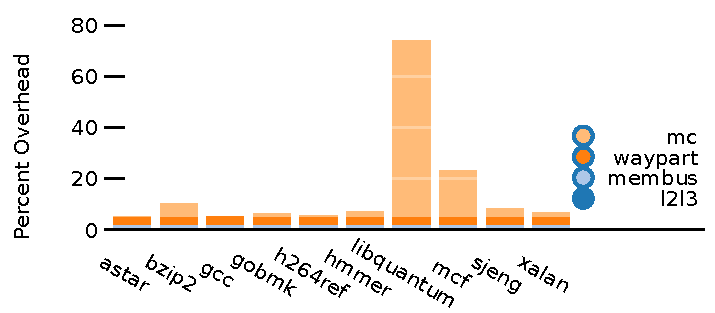
\includegraphics[width=3.4in]{figs/breakdown.pdf}
        \caption{Performance overhead for 2 TCs.}
        \label{fig:performance}
    \end{center}
\end{figure}

The performance overhead is likely to increase as the number of timing 
compartment scales up. To study the impact of the number of timing 
compartments, we evaluated the performance overhead with three and four timing 
compartments on a 4-core  processor, each occupying one core and private L1 and 
L2 caches. They share a 4MB L3 cache. We do not evaluate all permutations of 4 
benchmarks. Instead, we only evaluate the subset of these permutations where 
TC1, TC2, and TC3 are executing the same benchmark. As before, each of these 
workloads with the same program in TC0 is averaged.

The performance overhead as the number of timing compartments increases is 
shown in Figure~\ref{fig:scalability}. The arithmetic mean of the overheads for 
each benchmark for 2, 3 and 4 timing compartments are 9\%, 17\%, and 24\% 
respectively. For libquantum which is particularly memory intensive, the 
overheads are 76\%, 140\%, and 184\% for 2, 3, and 4 timing compartments. The 
results suggest that the overhead of timing timing channel protection is rather 
insensitive to the number of timing compartments for compute-bound 
applications. For memory-intensive applications, the overhead can increase 
noticeably. However, the results still suggest that timing compartments can 
allow distrusting software entities to share hardware and provide better 
overall performance than running them on separate dedicated machines.

\begin{figure}
    \begin{center}
        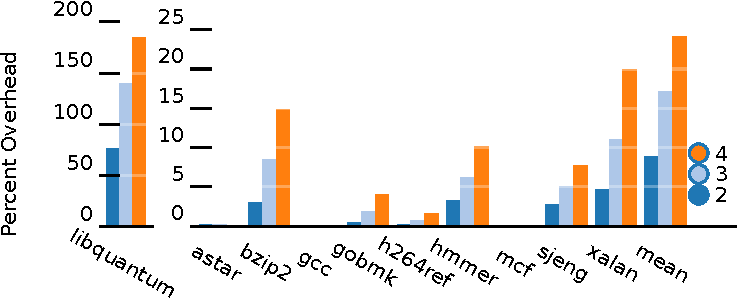
\includegraphics[width=3.4in]{figs/scalability_split.pdf}
        \caption{Performance overhead for 4 TCs.}
        \label{fig:scalability}
    \end{center}
\end{figure}

While future multi-core systems are likely to have a large number of processing 
cores, we note that many security applications will not require many timing 
compartments to be used concurrently. For example, the BYOD application only 
requires two TCs no matter how many cores exist in the system. Similarly, in 
a high-assurance cloud computing environment, the cloud provider can limit the
number of high-assurance virtual machines that can be located on each physical
system while increasing the system utilization by co-locating non-secure
virtual machines with high-assurance ones.


% \section{Related Work}

Previous studies identified 
a number of microarchitectural timing channels 
caches~\cite{percival,bernstein,caseofaes,remoteaes,analyticalcache,collision,
deconstructing,cachegames}, branch predictors 
\cite{branchpred,predictingbranch}, processor
pipelines \cite{pipelines}, networks on chip~\cite{yaonocs,surfnoc}, and memory
controllers~\cite{ushpca14,fletcher-hpca14}. 
Also, people have proposed solutions for timing channels in
individual components such as caches~\cite{newcache,deconstructing}, memory
controllers~\cite{ushpca14,fletcher-hpca14}, and on-chip network
~\cite{yaonocs,surfnoc}.
However, the previous work has
so far focused on individual component. This work represents the first attempt
at designing a full microprocessor with complete internal timing channel protection.
Our integration efforts also exposed new sources of timing channels in module
interfaces such as MSHRs and cache/memory response ports.

%However, this paper presents the first microarchitecture to address all 
%internal microarchitectural timing channels. 

Ascend~\cite{ascend} proposes a
microarchitecture that aims to eliminate external timing channels so that
even untrusted software can execute without leaking any confidential
data. This presents a powerful option if physical attacks need to be
considered. However, Ascend does not allow a processor to be shared by
multiple software components at the same time, and does not address 
any internal timing channels.
Execution leases~\cite{execution_leases} 
provide another external timing channel solution at the hardware level by 
enforcing strict upper bounds on the execution times of program subsections. 

Timing channels are a form of information flow, and many approaches to 
controlling timing channels are based in information flow theory. Language 
level approaches track information flow and to either 
eliminate~\cite{quantleaks} or 
reduce~\cite{mitigation1,mitigation2,mitigation3} timing channels. At the 
systems level, information flow has been used to provide security 
through explicit channels ~\cite{flume-sosp07,histar-sosp06,laminar-pldi09}. 
These can be combined with timing compartments to provide total software 
isolation.

Work has also been done to verify hardware timing channel protection. GLIFT 
\cite{glift-asplos09} tracks all information flows, (including timing channels) 
in hardware at the gate level, though it does so at a high cost. GLIFT has 
later been used to develop information flow property checkers in gate level 
simulators ~\cite{glift-dac10,glift-dac11,glift-isca11}, and more recently 
hardware description languages that verify timing channel securtity 
~\cite{caisson-plas10,caisson-pldi11,sapper-plas13}.

% \section{Conclusion}
This paper presents timing compartments, which provide an architecture 
abstraction to eliminate timing channels. When used in conjunction with access 
controls, timing compartments can provide total software-level isolation since 
other side or covert channel attacks require physical access. To realize 
timing compartments, we designed a full multiprocessor microarchitecture 
that eliminates all inter-program timing channels and evaluated it in the gem5 
architectural simulator. Our results show that the overheads are low.


%\bstctlcite{bstctl:etal, bstctl:nodash, bstctl:simpurl}
%\bibliographystyle{IEEEtranS}
 \bibliographystyle{abbrv}
%\bibliographystyle{latex8}
 \bibliography{paper}

\end{document}
